% =====================================================================
%  background.tex  --  Chapter 3 (Theoretical Background)
%
%  REVISION NOTE (this version):
%   1. This chapter is the HOME OF THE FORMAL DEFINITIONS of every
%      quantity that appears in more than one chapter: F_dH
%      (eq:fdh_definition), the burnup-to-EFPD conversion (eq:efpd),
%      reactivity (eq:reactivity) and Spearman's coefficient
%      (eq:spearman). The introduction describes them qualitatively and
%      points here. The methodology defines only its own constructs
%      (estimator, end-of-cycle criterion, k_target, constraints).
%   2. Every displayed formula is followed by a term-by-term list with
%      units.
%   3. Enumerations are set as lists. No semicolons, no em dashes.
%   4. Spearman's coefficient is written rho_S to avoid the collision
%      with reactivity rho.
%   5. Cross-references into the results chapter now point to the
%      existing labels sec:res-c1c2 and sec:res-corevalidation. The
%      variable-importance subsection still does not exist and remains
%      flagged.
%
%   6. Sections 3.7-3.9 restructured into ONE section, "The dual
%      optimisation process" (label sec:bg-moo kept), with subsections
%      hypervolume (sec:bg-hv), NSGA-II (sec:bg-nsga2), GP surrogates
%      (sec:bg-gp kept) and active-learning loop (sec:bg-al kept).
%      Each subsection: step-by-step theory with book citations, then
%      an "In this thesis" paragraph tying the theory to the concrete
%      parameters of the campaigns. Traditional-book citations added
%      to Sections 3.1-3.6. New entries in references_additions.bib.
%
%   7. 14 September 2026: split into short paragraphs for human
%      reading, every enumeration set as a LaTeX list. The cost of one
%      OpenMC evaluation in Section 3.7 now reads fifteen to
%      twenty-five minutes, as in the paragraph that follows it.
%
%   8. 15 September 2026: k balance, four- and six-factor formulas
%      (Duderstadt and Hamilton) in Section 3.1. The Bateman equations
%      moved here from the literature review, with power normalisation,
%      CE and CE/CM integration and CRAM after Romano et al. 2021 and
%      Pusa 2016 (sec:bg-bateman and following). Monte Carlo section
%      split into source iteration, tallies and estimators, and
%      statistics, with formulas from Lux and Koblinger and OpenMC
%      practice from Romano et al. 2015.
%
%  Figures: the eight ORIGINAL bg_*.pdf files (generated by
%  theoretical_background_figures.py). Requires graphicx, booktabs,
%  amsmath.
% =====================================================================

\providecommand{\openpoint}[1]{\par\noindent\fbox{\parbox{0.97\linewidth}{%
  \textbf{Open point:} #1}}\par}

\chapter{Theoretical Background}
\label{ch:background}

This chapter assembles the minimum theory the thesis rests on. The
equations are stated with the source in which each is derived, and the
derivations are not repeated. The emphasis falls on the points where
theory shapes decisions taken later.

The material is ordered as the methodology uses it:

\begin{enumerate}
  \item Neutron multiplication and its leakage hierarchy.
  \item Fuel depletion and the role of the burnable absorber.
  \item The power-peaking figure of merit.
  \item The Monte Carlo method and its statistical consequences.
  \item Reduced-order proxies and rank fidelity.
  \item The dual optimisation process, built from four components:
  \begin{enumerate}
    \item the hypervolume indicator,
    \item the NSGA-II search,
    \item the Gaussian-process surrogates, and
    \item the active-learning loop.
  \end{enumerate}
\end{enumerate}

This chapter also hosts the formal definitions of the quantities used
throughout the thesis. The choices that turn those definitions into
computable numbers are methodological and are fixed in
Chapter~\ref{ch:methodology}:

\begin{itemize}
  \item The estimator.
  \item The evaluation domain.
  \item The end-of-cycle criterion.
\end{itemize}

\section{Neutron multiplication, leakage and reactivity}
\label{sec:bg-k}

The multiplication factor is the ratio of the neutron populations in
successive fission generations. A more practical definition follows from
the neutron balance of the system~\cite{duderstadt_hamilton_1976}.

\begin{equation}
k = \frac{\text{rate of neutron production}}
         {\text{rate of neutron absorption} + \text{rate of neutron leakage}}
\label{eq:k-balance}
\end{equation}

\noindent where the symbols have the following meaning:

\begin{itemize}
  \item $k$ is the multiplication factor, dimensionless.

  \item The production rate is the rate at which fission releases
        neutrons in the system, in neutrons\,s$^{-1}$.

  \item The absorption and leakage rates are the rates at which neutrons
        are absorbed in the system and escape from it, in
        neutrons\,s$^{-1}$.
\end{itemize}

In an infinite system no neutron escapes, and the non-leakage
probability is one. For a thermal reactor the neutron life cycle then
splits the multiplication factor into four factors, known as the
four-factor formula~\cite{duderstadt_hamilton_1976}.

\begin{equation}
k_\infty = \eta\, f\, p\, \varepsilon
\label{eq:kinf}
\end{equation}

\noindent where the symbols have the following meaning:

\begin{itemize}
  \item $k_\infty$ is the infinite multiplication factor, dimensionless.

  \item $\eta$ is the thermal fission reproduction factor, the number of
        fission neutrons produced per thermal neutron absorbed in the
        fuel, dimensionless.

  \item $f$ is the thermal utilisation, the probability that an absorbed
        thermal neutron is absorbed in the fuel, dimensionless.

  \item $p$ is the resonance escape probability, the probability that a
        fast fission neutron slows down to thermal energies without being
        captured, notably in the resonances of $^{238}$U, dimensionless.

  \item $\varepsilon$ is the fast fission factor, the ratio of the fast
        neutrons produced by fast and thermal fission to those produced
        by thermal fission alone, dimensionless.
\end{itemize}

In a finite system some neutrons leak out while they slow down and some
after they have reached thermal energies. Each loss enters as a
non-leakage probability, which gives the six-factor formula for the
effective multiplication factor~\cite{duderstadt_hamilton_1976}.

\begin{equation}
k_\mathrm{eff} = k_\infty\, P_\mathrm{FNL}\, P_\mathrm{TNL}
= \eta\, f\, p\, \varepsilon\, P_\mathrm{FNL}\, P_\mathrm{TNL}
\label{eq:keff}
\end{equation}

\noindent where the symbols have the following meaning:

\begin{itemize}
  \item $k_\mathrm{eff}$ is the effective multiplication factor of the
        finite system, dimensionless.

  \item $P_\mathrm{FNL}$ is the fast non-leakage probability, the
        probability that a fast neutron does not leak out of the system,
        dimensionless.

  \item $P_\mathrm{TNL}$ is the thermal non-leakage probability, the
        probability that a thermal neutron does not leak out of the
        system, dimensionless.
\end{itemize}

Both probabilities are below one in a finite system, so $k_\mathrm{eff}$
is always smaller than $k_\infty$ for the same material composition. The
factors give a physical reading of the multiplication factor. In this
work $k$ itself is estimated directly by OpenMC from continuous-energy
transport over successive fission generations, as described in
Section~\ref{sec:bg-mc-k}.

Figure~\ref{fig:bg-k} shows this hierarchy measured on C9-47, one of the
designs of the Campaign 9 Pareto set, at beginning of life with all rods
out and the fixed soluble boron concentration of the campaign model. The
three-dimensional value falls below unity because that concentration
exceeds the critical one for this design, which is treated in
Section~\ref{sec:meth-boron}.

Each geometric step opens an additional leakage path. The
ratio of the core value to the assembly value defines the
leakage-corrected end-of-cycle target used throughout the optimisation:

\begin{itemize}
  \item Single assembly under reflective boundaries,
        $k_\infty = 1.11414 \pm 0.00071$, dimensionless, from two seeds
        of \num{10000} particles and 120 batches with 30 inactive.

  \item Two-dimensional core of 32 assemblies with reflector and vacuum
        outer boundary, $k_\mathrm{eff} = 1.02742 \pm 0.00015$,
        dimensionless, from two seeds of \num{150000} particles and 200
        batches with 80 inactive. The step of \SI{-7575}{pcm} measures
        the radial leakage of the finite core.

  \item Three-dimensional core of finite height with its structural
        components, namely the nozzles, end caps, plenum springs, spacer
        grids, control-rod stack, barrel, downcomer and vessel wall,
        $k_\mathrm{eff} = 0.99690 \pm 0.00015$, dimensionless, at the
        same fidelity. The further step is \SI{-2980}{pcm}.
\end{itemize}

\begin{figure}[htbp]
  \centering
  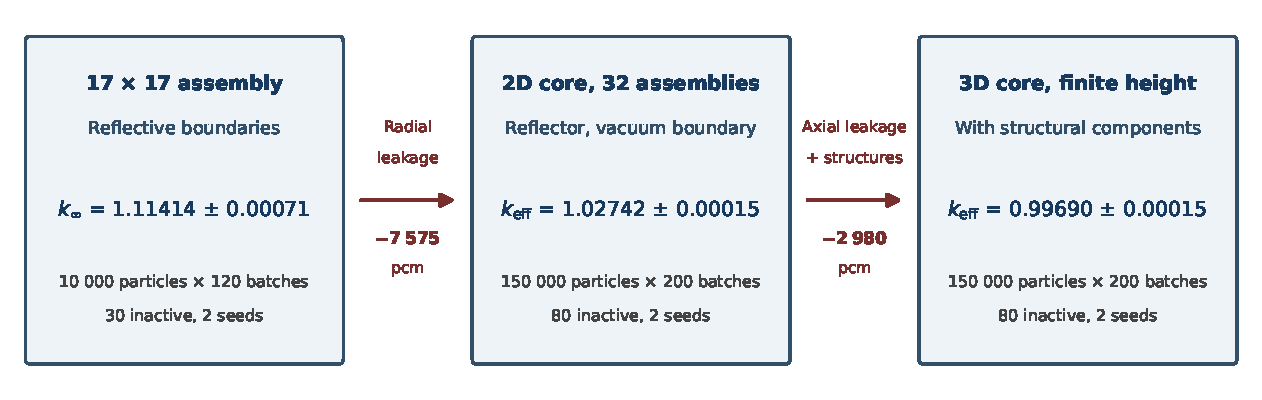
\includegraphics[width=0.92\linewidth]{images/bg_k_hierarchy.pdf}
  \caption{Multiplication ladder of C9-47, a design of the Campaign 9 Pareto set.}
  \label{fig:bg-k}
\end{figure}

Reactivity expresses the departure from criticality in a form that adds
linearly for small perturbations.

\begin{equation}
\rho = \frac{k - 1}{k}
\label{eq:reactivity}
\end{equation}

\noindent where the symbols have the following meaning:

\begin{itemize}
  \item $\rho$ is the reactivity, dimensionless, commonly reported in
        per cent mille (pcm), where $1~\mathrm{pcm} = 10^{-5}$.

  \item $k$ is the multiplication factor of the system under
        consideration, either $k_\infty$ or $k_\mathrm{eff}$,
        dimensionless.
\end{itemize}

Two competing requirements act on the beginning-of-life (BOL)
multiplication factor:

\begin{enumerate}
  \item It must exceed unity by enough margin that the core stays
        critical through the intended depletion history.

  \item It must remain bounded above, so that the excess reactivity can
        be held down by the available burnable absorber and control-rod
        worth.
\end{enumerate}

Both requirements enter the optimisation as explicit inequality
constraints on $k_\mathrm{BOL}$. The numerical bounds and their
evaluation level are given in Table~\ref{tab:constraints}.

A further consequence follows from the model level chosen for the
depletion. Because the depletion calculation is performed on the
\emph{assembly} under reflective boundaries, end of cycle cannot be
defined at $k_\infty = 1$.

The finite core that the assembly represents loses reactivity to
leakage, so the end-of-cycle criterion must be raised above unity by a
leakage correction. That correction is the target multiplication factor
formally defined in Section~\ref{sec:meth-ktarget}.

\section{Depletion, burnup and cycle length}
\label{sec:bg-depletion}

As fissile material is consumed and absorbing fission products
accumulate, the multiplication factor falls with burnup.

Burnup is the thermal energy released per unit mass of heavy metal
initially present, expressed in MWd/kgHM. It is the natural independent
variable of a depletion calculation because it is independent of the
power level at which the energy was produced.

The isotopic evolution obeys coupled rate equations of production,
decay and absorption for every nuclide~\cite{duderstadt_hamilton_1976},
known as the Bateman equations. They are solved here by the OpenMC
depletion module, with reaction rates updated by transport solutions on
an adaptive burnup schedule. The equations and the method of solution
are given in Section~\ref{sec:bg-bateman}.

The depletion runs at constant power, normalised to the heavy-metal
mass loaded at beginning of life, and burnup is referred to that same
initial mass. The specific power $P_\mathrm{spec}$ is therefore constant
by construction, and burnup grows linearly with irradiation time,
$B = P_\mathrm{spec}\,t/10^{3}$ with $t$ in days~\cite{lee_2020}.
Cycle length is
therefore reported in effective full-power days (EFPD), obtained from
the end-of-cycle burnup through the conversion below.

\begin{equation}
\mathrm{EFPD} = \frac{10^{3}\,B_\mathrm{EOC}}{P_\mathrm{spec}}
\label{eq:efpd}
\end{equation}

\noindent where the symbols have the following meaning:

\begin{itemize}
  \item $\mathrm{EFPD}$ is the cycle length in effective full-power
        days, in days.

  \item $B_\mathrm{EOC}$ is the end-of-cycle burnup, in MWd/kgHM.

  \item $P_\mathrm{spec}$ is the specific power of the fuel, in
        W\,g$^{-1}$ of heavy metal, numerically equal to
        kW\,kg$^{-1}$ of heavy metal.

  \item $10^{3}$ converts megawatt-days into kilowatt-days, so that the
        ratio closes to days.
\end{itemize}

The numerator is strictly the burnup increment accumulated over the
cycle, $B_\mathrm{EOC} - B_\mathrm{BOC}$. It reduces to
$B_\mathrm{EOC}$ here because the core is a fresh, uniform,
single-batch loading, so the beginning-of-cycle burnup is zero. A
multi-batch core would require the increment in its place.

The criterion that fixes the end-of-cycle burnup $B_\mathrm{EOC}$ is a
methodological choice. The criterion used in this work, together with
the treatment of the discharge-burnup limit, is defined in
Section~\ref{sec:objective_functions}.

Figure~\ref{fig:bg-dep} illustrates how $k_\infty$ of an assembly
evolves with burnup, using three designs of this work that differ in
enrichment and gadolinia loading. Three features of such curves matter
for the optimisation:

\begin{enumerate}
  \item The reactivity-defined end of cycle, reached where $k_\infty$
        crosses the leakage-corrected target of
        Section~\ref{sec:meth-ktarget}. A higher enrichment moves the
        crossing to a higher burnup and lengthens the cycle.

  \item The gadolinia hold-down and its burnout. A large gadolinia load
        holds $k_\infty$ down at the start of life, and its burnout then
        raises $k_\infty$ to a peak before fuel depletion takes over. A
        small load leaves no visible rise, and $k_\infty$ falls
        throughout the cycle after the initial xenon drop.

  \item The discharge-burnup limit of the fuel, which ends irradiation
        whenever the reactivity crossing lies beyond it, so the cycle
        length of a highly enriched design is set by the limit instead
        of by reactivity. The curves are assembly-average burnup, so the
        figure marks the assembly-average limit of \SI{55}{MWd/kgHM} of
        uranium dioxide in zirconium cladding~\cite{song_sanchez_2026}.
        The limit adopted for the accident-tolerant fuel of this work is
        defined in Section~\ref{sec:meth-atf}.
\end{enumerate}

\begin{figure}[htbp]
  \centering
  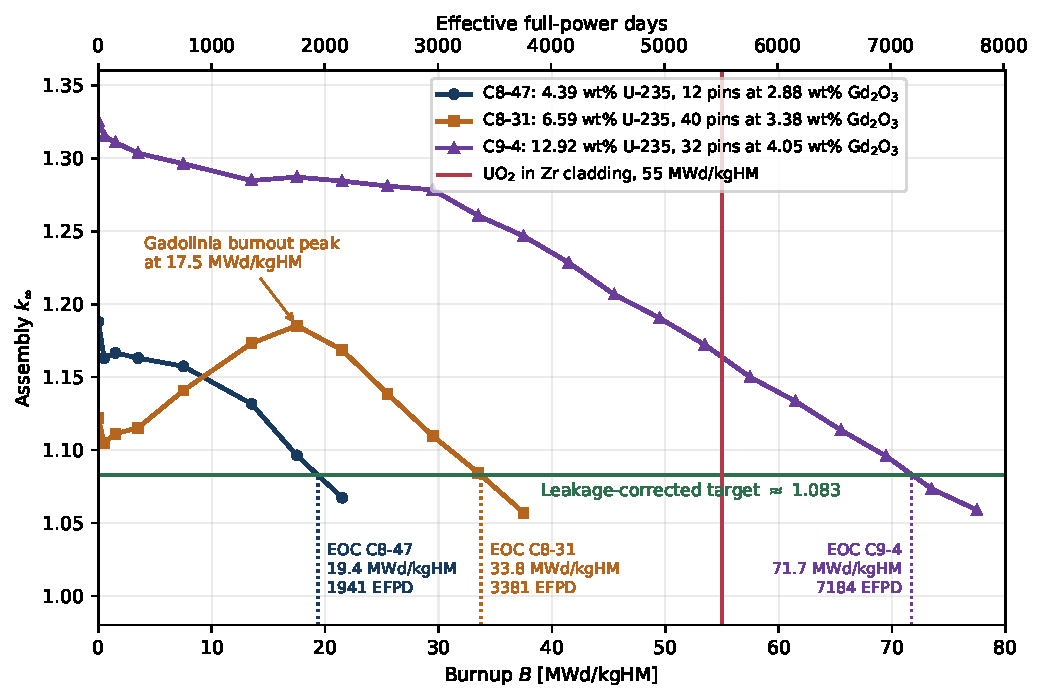
\includegraphics[width=0.9\linewidth]{images/bg_gd_depletion.pdf}
  \caption{Assembly life curves of designs C8-47, C8-31 and C9-4.}
  \label{fig:bg-dep}
\end{figure}

\subsection{The depletion equations}
\label{sec:bg-bateman}

The depletion calculations of this work follow the formulation of the
OpenMC depletion module~\cite{romano_2021_depletion}. The density of
each nuclide rises through production from other nuclides, by
transmutation and by decay, and falls through its own transmutation and
decay. Written for every nuclide, this balance gives the Bateman
equations~\cite{romano_2021_depletion}.

\begin{equation}
\begin{split}
\frac{\mathrm{d}N_i(t)}{\mathrm{d}t} = {} &
\sum_{j=1}^{n}\left[\int_0^\infty \mathrm{d}E\,
f_{j\rightarrow i}(E)\,\sigma_j(E,t)\,\phi(E,t)
+ \lambda_{j\rightarrow i}\right] N_j(t) \\
& - \left[\int_0^\infty \mathrm{d}E\,\sigma_i(E,t)\,\phi(E,t)
+ \sum_{j=1}^{n}\lambda_{i\rightarrow j}\right] N_i(t),
\qquad i = 1,\dots,n
\end{split}
\label{eq:bateman}
\end{equation}

\noindent where the symbols have the following meaning:

\begin{itemize}
  \item $N_i(t)$ and $N_j(t)$ are the densities of nuclides $i$ and $j$
        at time $t$, in atoms\,cm$^{-3}$.

  \item $t$ is the time, in s.

  \item $E$ is the neutron energy, in eV.

  \item $\phi(E,t)$ is the neutron flux at energy $E$ and time $t$, in
        cm$^{-2}$\,s$^{-1}$\,eV$^{-1}$.

  \item $\sigma_i(E,t)$ is the transmutation cross section of nuclide
        $i$, the sum of the cross sections of all reaction channels that
        transmute it, in cm$^{2}$.

  \item $f_{j\rightarrow i}(E)$ is the fraction of the transmutation
        reactions of nuclide $j$ that produce nuclide $i$,
        dimensionless.

  \item $\lambda_{j\rightarrow i}$ is the decay constant of the decay
        modes of nuclide $j$ that produce nuclide $i$, in s$^{-1}$.

  \item $n$ is the total number of nuclides, dimensionless.
\end{itemize}

By definition $f_{i\rightarrow i}$ and $\lambda_{i\rightarrow i}$ are
zero, so the sums run over all nuclides except $i$. The initial
densities $N_i(0) = N_{i,0}$ close the system. Collecting the $n$
densities into one vector gives the matrix
form~\cite{romano_2021_depletion}.

\begin{equation}
\frac{\mathrm{d}\mathbf{n}}{\mathrm{d}t} =
\mathbf{A}(\mathbf{n})\,\mathbf{n},
\qquad \mathbf{n}(0) = \mathbf{n}_0
\label{eq:bateman-matrix}
\end{equation}

\noindent where the symbols have the following meaning:

\begin{itemize}
  \item $\mathbf{n}$ is the vector of nuclide densities, with components
        in atoms\,cm$^{-3}$, and $\mathbf{n}_0$ is its initial value.

  \item $\mathbf{A}(\mathbf{n})$ is the burnup matrix, whose entries are
        the bracketed coefficients of Equation~\eqref{eq:bateman}, in
        s$^{-1}$.
\end{itemize}

The matrix depends on the composition. Evaluating $\mathbf{A}$ for a
given composition amounts to solving the neutron transport equation for
the transmutation reaction rates and combining them with decay and
fission product yield data~\cite{romano_2021_depletion}. The system is
therefore nonlinear, and every evaluation of the matrix costs one
transport solution.

\subsection{Reaction rates and power normalisation}
\label{sec:bg-dep-norm}

OpenMC obtains the reaction rates of Equation~\eqref{eq:bateman} by
tallying them directly in each depleted material. A tally can be scored
with an analog, a collision or a track-length estimator
(Section~\ref{sec:bg-mc-tally}). The depletion module does not set an
estimator on its reaction-rate tally, which carries only material
filters and reaction scores, so OpenMC applies its default track-length
estimator~\cite{romano_2021_depletion,openmc_docs}. The tallied rates are expressed in reactions per source particle, while
the depletion needs absolute rates in reactions per second.

The conversion uses the total heating observed in the system. The ratio
of the system power to the observed heating is applied as a
normalisation factor to every reaction
rate~\cite{romano_2021_depletion}.

\begin{equation}
R_{i,x} = \frac{P}{H}\,\hat{R}_{i,x}
\label{eq:dep-norm}
\end{equation}

\noindent where the symbols have the following meaning:

\begin{itemize}
  \item $R_{i,x}$ is the absolute rate of reaction $x$ in nuclide $i$,
        in reactions\,s$^{-1}$.

  \item $\hat{R}_{i,x}$ is the tallied rate of the same reaction, in
        reactions per source particle.

  \item $P$ is the system power, in W. In this work it is the product of
        the specific power $P_\mathrm{spec}$ of Equation~\eqref{eq:efpd}
        and the fresh heavy-metal mass of the model, held constant
        through the cycle.

  \item $H$ is the heating observed in the system, in J per source
        particle.
\end{itemize}

The observed heating can be determined in two
ways~\cite{romano_2021_depletion}:

\begin{enumerate}
  \item From the fission reaction rates, each multiplied by a constant
        energy release per fission (Q value) taken from the depletion
        chain file.

  \item From a tally of the actual heating rate over the whole system.
\end{enumerate}

The depletion operator of this work leaves the normalisation mode at the
default of the OpenMC coupled operator, which is the first option. The
energy released per fission therefore enters every depletion through the
Q values of the chain file.

\subsection{Integration over a time step}
\label{sec:bg-dep-integ}

For a matrix held constant, Equation~\eqref{eq:bateman-matrix} has an
exact solution in the form of a matrix
exponential~\cite{romano_2021_depletion}.

\begin{equation}
\mathbf{n}(t) = \exp(\mathbf{A}t)\,\mathbf{n}_0,
\qquad
\exp(\mathbf{X}) = \sum_{m=0}^{\infty}\frac{\mathbf{X}^{m}}{m!}
\label{eq:mat-exp}
\end{equation}

\noindent where the symbols have the following meaning:

\begin{itemize}
  \item $\exp(\cdot)$ is the matrix exponential.

  \item $\mathbf{X}$ is a square matrix, with $\mathbf{X}^{0}$ equal to
        the identity matrix $\mathbf{I}$.

  \item $m$ is the summation index, dimensionless.
\end{itemize}

Since the matrix depends on the composition, the exponential is applied
step by step with an approximation of the matrix over each step. The
simplest numerical method, constant extrapolation (CE), holds the matrix
constant over the step at its value at the start of the
step~\cite{romano_2021_depletion}.

\begin{equation}
\mathbf{n}_{i+1} = \exp\!\big(h\,\mathbf{A}(\mathbf{n}_i)\big)\,\mathbf{n}_i
\label{eq:dep-ce}
\end{equation}

\noindent where the symbols have the following meaning:

\begin{itemize}
  \item $\mathbf{n}_i$ and $\mathbf{n}_{i+1}$ are the compositions at
        the start and at the end of step $i$, in atoms\,cm$^{-3}$. Here
        the index $i$ counts time steps, not nuclides.

  \item $h$ is the length of the step, in s.
\end{itemize}

The CE method needs a single transport solution and a single matrix
exponential per step, and it is only first-order accurate, with an error
that converges as $\mathcal{O}(h)$~\cite{romano_2021_depletion}. It is
the scheme of the \texttt{PredictorIntegrator} class of OpenMC, which
every depletion of this work uses. Its accuracy is therefore governed by
the length of the steps, which the burnup schedule of
Chapter~\ref{ch:methodology} fixes.

Higher accuracy is obtained by evaluating the matrix again inside the
step. The constant extrapolation, constant midpoint (CE/CM) method first
advances the composition to the middle of the step and then uses the
matrix at the midpoint over the whole step~\cite{romano_2021_depletion}.

\begin{equation}
\begin{aligned}
\mathbf{n}_{i+1/2} &= \exp\!\left(\tfrac{h}{2}\,\mathbf{A}(\mathbf{n}_i)\right)\mathbf{n}_i \\
\mathbf{n}_{i+1} &= \exp\!\big(h\,\mathbf{A}(\mathbf{n}_{i+1/2})\big)\,\mathbf{n}_i
\end{aligned}
\label{eq:dep-cecm}
\end{equation}

\noindent where $\mathbf{n}_{i+1/2}$ is the composition at the middle of
step $i$, in atoms\,cm$^{-3}$. The CE/CM method requires two transport
solutions and two matrix exponentials per step, twice the cost of the CE
method, and it is second-order accurate~\cite{romano_2021_depletion}.

The OpenMC depletion module offers further schemes of the same
family~\cite{romano_2021_depletion}:

\begin{itemize}
  \item Constant extrapolation with linear interpolation (CE/LI) and
        linear extrapolation with quadratic interpolation (LE/QI), which
        interpolate the matrix between the start and the end of the
        step.

  \item The fourth-order Lie group integrator CF4, with four transport
        solutions per step, which allows long steps without loss of
        accuracy.

  \item The classic fourth-order Runge--Kutta method written in
        exponential form.

  \item Stochastic implicit versions of the CE, CE/LI and LE/QI methods.
\end{itemize}

All the explicit schemes are only conditionally stable, and oscillating
and diverging solutions have been observed with them. The stochastic
implicit method of Dufek et al.\ is unconditionally stable but, like the
CE method, only first-order accurate~\cite{romano_2021_depletion}. The
consequences of this instability for Monte Carlo depletion are discussed
in Section~\ref{sec:lit-opt-burnup}.

\subsection{The matrix exponential by CRAM}
\label{sec:bg-dep-cram}

Every scheme above needs the exponential of a burnup matrix, and burnup
matrices are hard for general-purpose methods. The decay constants vary
so widely that the short-lived nuclides produce eigenvalues with
absolute values up to the order of $10^{21}$, and depletion steps range
from a few days to several months. Methods built on an approximation
near the origin, such as the truncated Taylor series or the Pad\'e
approximation, work well only when the norm of $\mathbf{A}t$ is small,
which is not the case for burnup matrices~\cite{pusa_2016}.

The Chebyshev rational approximation method (CRAM) replaces the
exponential with its best rational approximation on the negative real
axis~\cite{pusa_2016}. OpenMC evaluates it in the incomplete partial
fraction form~\cite{romano_2021_depletion}.

\begin{equation}
\exp(\mathbf{A}t) \approx \alpha_0 \prod_{l=1}^{q/2}
\left(\mathbf{I} + 2\,\mathrm{Re}\!\left[\tilde{\alpha}_l\,
(\mathbf{A}t - \theta_l\mathbf{I})^{-1}\right]\right)
\label{eq:cram}
\end{equation}

\noindent where the symbols have the following meaning:

\begin{itemize}
  \item $q$ is the order of the approximation, an even number,
        dimensionless.

  \item $\alpha_0$ is the limit of the rational approximation at
        infinity, dimensionless.

  \item $\theta_l$ are the poles of the approximation, complex and
        dimensionless.

  \item $\tilde{\alpha}_l$ are the residues of its degree-two factors,
        complex and dimensionless.

  \item $\mathrm{Re}[\cdot]$ is the real part, and $\mathbf{I}$ is the
        identity matrix.
\end{itemize}

Each factor of the product requires the solution of one sparse linear
system, so an approximation of order $q$ requires $q/2$ solutions.
OpenMC uses order 48 by default, which means 24 sparse linear systems for
each matrix exponential~\cite{romano_2021_depletion}. For a burnup system
of 1606 nuclides and a step of ten days, order 16 already gives maximum
relative errors of the order of $10^{-5}$, while pure decay calculations
need higher orders~\cite{pusa_2016}.

\section{Power peaking}
\label{sec:bg-peaking}

Thermal margins are governed by the power of the hottest fuel rod, and
the core average says little about them.

A thermal design margin is the allowance kept between the operating
limits and the limits at which the fuel or the cladding fails. The
thermal design limits of a pressurised water reactor are set on three
mechanisms~\cite{todreas_kazimi_2012}:

\begin{enumerate}
  \item Departure from nucleate boiling, in which the well-behaved
        bubble formation on the cladding surface gives way to a
        continuous vapour film. Because steam conducts heat poorly, the
        cladding temperature then rises by hundreds of kelvin within
        seconds. This is the governing limit in normal operation.

  \item Melting of the fuel pellet centre, which is the hottest point
        of the core.

  \item The peak cladding temperature reached during a loss-of-coolant
        accident, which depends on the energy stored in the hottest rod
        when the transient begins.
\end{enumerate}

All three are properties of the single most heavily loaded rod. A
neutronic power distribution over several hundred rods must therefore be
reduced to a figure of merit that expresses how much worse that rod is
than the mean. The radial peaking factor $F_{\Delta H}$ is the figure of
merit used in this work for that purpose.

The connection to the first mechanism is direct. The enthalpy rise of
the coolant along a channel is proportional to the total power added
along it, which is the axially integrated power of the adjacent
rod~\cite{todreas_kazimi_2012}.

A channel with a high $F_{\Delta H}$ therefore reaches the boiling
crisis at a lower core power. Flattening the radial power distribution
buys margin that can be spent on power output or on cycle length.

The radial peaking factor is defined as the ratio between the axially
integrated linear power of the most heavily loaded fuel rod and the
average axially integrated linear power of all fuel rods in the
evaluation domain.

\begin{equation}
F_{\Delta H}
=
\frac{\displaystyle \max_{i \in \{1,\dots,N\}} \int_{0}^{H} q'_i(z)\,\mathrm{d}z}
     {\displaystyle \frac{1}{N} \sum_{j=1}^{N} \int_{0}^{H} q'_j(z)\,\mathrm{d}z}
\label{eq:fdh_definition}
\end{equation}

\noindent where the symbols have the following meaning:

\begin{itemize}
  \item $F_{\Delta H}$ is the radial peaking factor, dimensionless,
        equal to unity for a perfectly flat radial power distribution.

  \item $q'_i(z)$ is the linear power density of fuel rod $i$ at axial
        elevation $z$, in W\,cm$^{-1}$.

  \item $z$ is the axial coordinate measured from the bottom of the
        active fuel region, in cm.

  \item $H$ is the active fuel height, in cm.

  \item $N$ is the number of fuel rods in the evaluation domain,
        dimensionless.

  \item $i$ and $j$ are fuel rod indices, dimensionless.
\end{itemize}

The factor is a thermal-hydraulic margin indicator expressed in purely
neutronic terms. That is what allows it to serve as an objective in a
model without thermal-hydraulic feedback.

Two methodological choices remain, and both are fixed in
Section~\ref{sec:objective_functions}:

\begin{itemize}
  \item The evaluation domain over which the maximum is taken.

  \item The Monte Carlo estimator that replaces the integrals in
        practice.
\end{itemize}

Figures~\ref{fig:bg-pin-asm} and~\ref{fig:bg-pin-core} illustrate the
radial peaking factor on C9-47, one of the designs of the Campaign 9
Pareto set, at beginning of life. Each map shows the fission rate of every pin divided by the mean
over the fuelled pins, so $F_{\Delta H}$ is the largest value of the
map.

In the assembly with reflective boundaries of
Figure~\ref{fig:bg-pin-asm}, only the lattice shapes the distribution:

\begin{itemize}
  \item The pins next to the guide tubes, grey in the figure, receive
        extra moderation and carry the highest powers.

  \item The gadolinia-bearing pins, ringed in the figure, fall to about
        one third of the mean.
\end{itemize}

\begin{figure}[htbp]
  \centering
  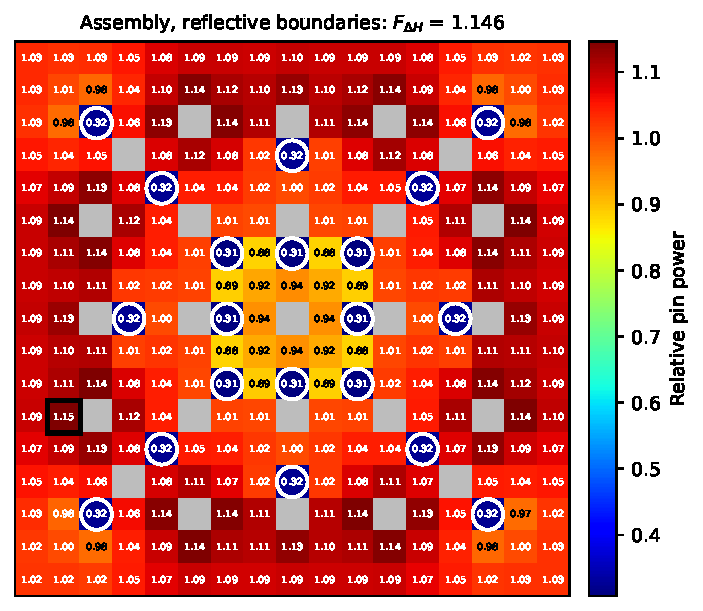
\includegraphics[width=0.60\linewidth]{images/bg_pin_power_asm.pdf}
  \caption{Relative pin power of the C9-47 assembly under reflective boundaries.}
  \label{fig:bg-pin-asm}
\end{figure}

The factor of this assembly is 1.146. In the core of
Figure~\ref{fig:bg-pin-core}, the same lattice pattern is superimposed
on the radial power shape of the finite core. Pins next to the reflector
lose neutrons to leakage, and the enrichment zoning of
Section~\ref{sec:meth-zoning} moves the peak from the centre to the
surrounding ring of assemblies, so the factor rises to 1.515. The
hottest pin is never a gadolinia-bearing pin, so a maximum-based factor
does not register the absorber directly.

\begin{figure}[htbp]
  \centering
  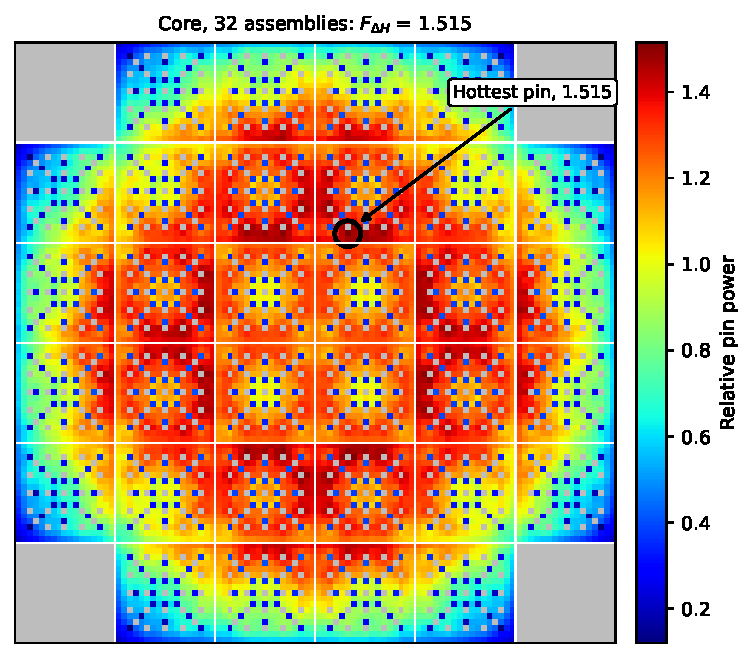
\includegraphics[width=0.64\linewidth]{images/bg_pin_power_core.pdf}
  \caption{Relative pin power of the C9-47 two-dimensional core.}
  \label{fig:bg-pin-core}
\end{figure}

Two properties of the figure of merit matter for the chapters that
follow:

\begin{enumerate}
  \item It is evaluated at beginning of life on fresh fuel, where
        enrichment zoning and absorber effects on the power
        distribution are strongest.

  \item It is a \emph{maximum over many estimated quantities}. Under
        Monte Carlo evaluation this makes it an extreme order
        statistic, with the statistical consequences developed in
        Section~\ref{sec:bg-mc}.
\end{enumerate}

\FloatBarrier

\section{Gadolinia burnable absorbers}
\label{sec:bg-gd}

Excess beginning-of-life reactivity must be held down without spending
control-rod worth~\cite{lee_2020}. Gadolinia (Gd$_2$O$_3$) mixed into
selected fuel pins achieves this
through the extreme thermal absorption of $^{155}$Gd and $^{157}$Gd.
That absorption is two to five orders of magnitude stronger than that of
the fuel nuclides, as shown in Figure~\ref{fig:bg-xs} with data from the
ENDF/B-VII.1 library used for every transport solve of this
work~\cite{chadwick_endf71_2011}.

Poisoned pellets are optically black to thermal neutrons, so absorption
proceeds from the pellet surface inward. The \emph{duration} of the
hold-down is therefore set by geometry as much as by absorber content.

Industrial practice exploits this self-shielding by concentrating the
poison in a limited number of rods~\cite{gd_enriched_2021}.

Three consequences recur in the results of this thesis:

\begin{enumerate}
  \item The number of poisoned pins sets the initial hold-down, because
        each pin absorbs from its surface, while the concentration
        within the pin sets how long the absorber
        lasts~\cite{alam_partI_2019}. The total inventory bounds the
        achievable hold-down, but the reactivity worth of the
        burnable absorber is not a function of the product of
        concentration and pin count alone.

  \item The residual end-of-life reactivity penalty of natural
        gadolinia is small~\cite{ba_snf_2001}.

  \item The local power depression couples the absorber to the peaking
        objective in a way that a maximum-based estimator cannot
        register. The absorber lowers the power of its own pin, and the
        estimator reads the hottest pin.
\end{enumerate}

\begin{figure}[htbp]
  \centering
  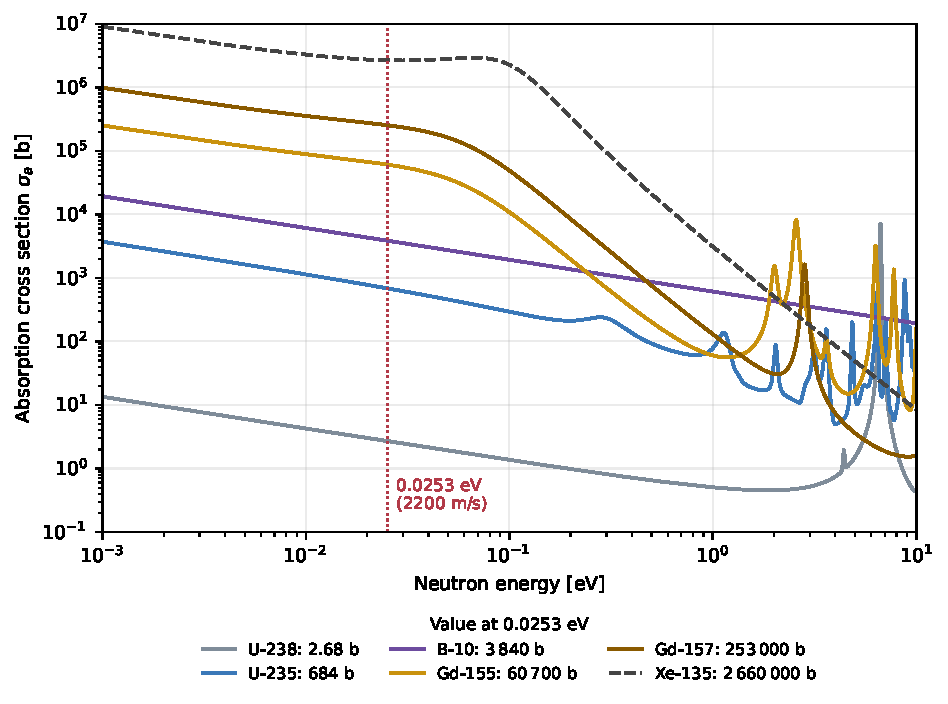
\includegraphics[width=0.8\linewidth]{images/bg_thermal_xs.pdf}
  \caption{Absorption cross sections at 294\,K from ENDF/B-VII.1.}
  \label{fig:bg-xs}
\end{figure}

\section{The Monte Carlo method and its statistics}
\label{sec:bg-mc}

OpenMC solves the transport problem by the Monte Carlo method. It follows
individual neutron histories through the geometry and scores the
quantities of interest on the events of those
histories~\cite{romano_openmc_2015}. Three parts of the method matter
for this thesis:

\begin{enumerate}
  \item The source iteration that estimates the multiplication factor
        (Section~\ref{sec:bg-mc-k}).

  \item The tallies and the estimators that score reaction rates
        (Section~\ref{sec:bg-mc-tally}).

  \item The statistics of the resulting estimates
        (Section~\ref{sec:bg-mc-stats}).
\end{enumerate}

\subsection{Source iteration and the multiplication factor}
\label{sec:bg-mc-k}

Monte Carlo estimates of the multiplication factor rest on source
iteration over successive fission generations~\cite{lux_koblinger_1991}.
OpenMC solves the $k$-eigenvalue problem by this method of successive
generations and lets several generations be grouped into a batch, which
reduces the correlation between realisations of the tally random
variables~\cite{romano_openmc_2015}. The calculation proceeds in
batches:

\begin{enumerate}
  \item A batch of neutron histories is tracked.

  \item The fission sites it produces seed the next batch.

  \item The earlier \emph{inactive} batches are discarded while the
        fission source is still settling.

  \item Tallies accumulate over the \emph{active} batches only.
\end{enumerate}

In a generation started from $N$ fission points, the estimate of the
multiplication factor is the number of fission points that the
generation produces per starting point~\cite{lux_koblinger_1991}.

\begin{equation}
\tilde{k}_g = \frac{N_g}{N}
\label{eq:mc-kn}
\end{equation}

\noindent where the symbols have the following meaning:

\begin{itemize}
  \item $\tilde{k}_g$ is the estimate of the multiplication factor in
        generation $g$, dimensionless.

  \item $N$ is the number of fission points that start each generation,
        dimensionless.

  \item $N_g$ is the number of fission points produced in generation
        $g$, dimensionless.
\end{itemize}

The first generations carry the bias of the initial source guess and are
discarded. The estimate of the multiplication factor is the average over
the remaining active generations~\cite{lux_koblinger_1991}.

\begin{equation}
\bar{k} = \frac{1}{G - G_\mathrm{in}}
\sum_{g=G_\mathrm{in}+1}^{G} \tilde{k}_g
\label{eq:mc-kbar}
\end{equation}

\noindent where the symbols have the following meaning:

\begin{itemize}
  \item $\bar{k}$ is the estimate of the multiplication factor,
        dimensionless.

  \item $G$ is the total number of generations, dimensionless.

  \item $G_\mathrm{in}$ is the number of inactive generations discarded
        at the start, dimensionless.
\end{itemize}

OpenMC keeps the collision, absorption and track-length estimators of
$k_\mathrm{eff}$ side by side and reports a minimum-variance combination
of the three, based on their covariance
matrix~\cite{romano_openmc_2015}. Source convergence is monitored
through the Shannon entropy of the fission source. A structured mesh
covering at least all the fissionable materials is superimposed on the
geometry, and the fraction of source sites in each mesh element is
counted~\cite{openmc_docs}.

\begin{equation}
H = -\sum_{i=1}^{N_\mathrm{m}} S_i \log_2 S_i,
\qquad
S_i = \frac{\text{source sites in mesh element } i}
           {\text{total number of source sites}}
\label{eq:shannon}
\end{equation}

\noindent where the symbols have the following meaning:

\begin{itemize}
  \item $H$ is the Shannon entropy of the fission source, in bits.

  \item $N_\mathrm{m}$ is the number of mesh elements, dimensionless.

  \item $S_i$ is the fraction of the source sites that lie in mesh
        element $i$, dimensionless.
\end{itemize}

The mesh of this work has 8 by 8 by 1 elements
(Appendix~\ref{app:model-inputs}). The entropy becomes stationary once
the spatial source has settled.

The entropy is recorded for every evaluation from Campaign~3 onward as a
source-convergence diagnostic. The diagnostic does not stop or repeat an
evaluation inside the loop. The core solves are instead given 60 to 120
inactive batches, and the designs whose source had not converged when
the active batches began are identified afterwards
(Sections~\ref{sec:res-corevalidation}, \ref{sec:res-c7-limits}
and~\ref{sec:res-c8-limits}).

\subsection{Tallies and estimators}
\label{sec:bg-mc-tally}

Every physical result of an OpenMC run is obtained from a tally. A tally
is defined by a combination of filters and
scores~\cite{romano_openmc_2015}:

\begin{itemize}
  \item A filter limits the events that can score to the tally, based on
        attributes of the particle such as the cell it travels in or its
        pre-collision energy.

  \item A score names the physical quantity recorded for an event that
        passes the filters, such as the flux, the fission reaction rate
        or the energy deposited by fission.
\end{itemize}

Most scores are reaction rates integrated over a region of the
geometry~\cite{lux_koblinger_1991}.

\begin{equation}
R_x = \int_V \mathrm{d}\mathbf{r} \int_0^\infty \mathrm{d}E\,
\phi(\mathbf{r},E)\,\Sigma_x(\mathbf{r},E)
\label{eq:mc-rr}
\end{equation}

\noindent where the symbols have the following meaning:

\begin{itemize}
  \item $R_x$ is the rate of reaction $x$ in the region $V$, in
        reactions\,s$^{-1}$.

  \item $V$ is the region of the geometry, in cm$^{3}$, and
        $\mathbf{r}$ is the position, in cm.

  \item $E$ is the neutron energy, in eV.

  \item $\phi(\mathbf{r},E)$ is the scalar neutron flux, in
        cm$^{-2}$\,s$^{-1}$\,eV$^{-1}$.

  \item $\Sigma_x(\mathbf{r},E)$ is the macroscopic cross section of
        reaction $x$, in cm$^{-1}$.
\end{itemize}

A Monte Carlo run estimates this integral from the histories it
simulates, and OpenMC offers three estimators for it~\cite{openmc_docs}:

\begin{itemize}
  \item The analog estimator counts the reactions that actually occur
        in the region.

  \item The collision estimator scores at every collision in the
        region, whatever reaction takes place.

  \item The track-length estimator scores along every flight segment
        of the particle inside the region.
\end{itemize}

The collision estimator scores more events than the analog estimator,
each with a smaller contribution~\cite{openmc_docs}. At every collision
inside the region it scores the ratio of the reaction cross section to
the total cross section at the collision point~\cite{lux_koblinger_1991}.

\begin{equation}
\bar{R}_x^\mathrm{col} = \frac{1}{N_h} \sum_{c=1}^{n_c} w_c\,
h_V(\mathbf{r}_c)\,
\frac{\Sigma_x(\mathbf{r}_c,E_c)}{\Sigma_t(\mathbf{r}_c,E_c)}
\label{eq:mc-col}
\end{equation}

\noindent where the symbols have the following meaning:

\begin{itemize}
  \item $\bar{R}_x^\mathrm{col}$ is the collision estimate of the
        reaction rate, in reactions per source particle.

  \item $N_h$ is the number of simulated histories, dimensionless, and
        $n_c$ is the number of collisions in all of them, dimensionless.

  \item $w_c$ is the statistical weight of the particle entering
        collision $c$, dimensionless.

  \item $\mathbf{r}_c$ and $E_c$ are the position, in cm, and the energy,
        in eV, of the particle entering collision $c$.

  \item $h_V(\mathbf{r}_c)$ equals one when $\mathbf{r}_c$ lies in the
        region $V$ and zero otherwise, dimensionless.

  \item $\Sigma_t$ is the total macroscopic cross section, in cm$^{-1}$.
\end{itemize}

The track-length estimator scores along every flight segment that
crosses the region, with the length of the segment inside
it~\cite{lux_koblinger_1991}.

\begin{equation}
\bar{R}_x^\mathrm{tl} = \frac{1}{N_h} \sum_{s=1}^{n_s} w_s\, l_s\,
\Sigma_x(E_s)
\label{eq:mc-tl}
\end{equation}

\noindent where the symbols have the following meaning:

\begin{itemize}
  \item $\bar{R}_x^\mathrm{tl}$ is the track-length estimate of the
        reaction rate, in reactions per source particle.

  \item $n_s$ is the number of flight segments in all histories,
        dimensionless.

  \item $w_s$ is the statistical weight of the particle on segment $s$,
        dimensionless.

  \item $l_s$ is the length of segment $s$ inside the region $V$, in cm.

  \item $E_s$ is the energy of the particle on segment $s$, in eV, at
        which $\Sigma_x$ of the material of the region is evaluated.
\end{itemize}

The collision and track-length estimators are both unbiased estimates of the same quantity and can be evaluated
from the same set of histories~\cite{lux_koblinger_1991}. OpenMC writes
the two estimators in the same form, normalised by the total starting
weight of the particles in place of the number of
histories~\cite{openmc_docs}.

Its tallies are scored with the
track-length estimator by default~\cite{romano_openmc_2015}. A
track-length estimator cannot serve a tally that needs the state of the
particle after a collision, so tallies with outgoing-energy filters,
scattering change-in-angle filters or scattering moments use an analog
estimator~\cite{openmc_docs}. The reaction rates
that drive the depletion of Section~\ref{sec:bg-dep-norm} are
track-length estimates, because the depletion tally sets no estimator
and the default applies~\cite{romano_2021_depletion,openmc_docs}.

\subsection{Statistics of the estimates}
\label{sec:bg-mc-stats}

The active batches of a run give repeated estimates of every tally. For
$B$ batches, the result and its uncertainty are estimated by the sample
mean and by the sample variance of the mean~\cite{lux_koblinger_1991}.

\begin{equation}
\hat{x} = \frac{1}{B}\sum_{b=1}^{B}\bar{x}_b,
\qquad
s_{\hat{x}}^2 = \frac{1}{B(B-1)}\sum_{b=1}^{B}
\left(\bar{x}_b - \hat{x}\right)^2
\label{eq:mc-mean-var}
\end{equation}

\noindent where the symbols have the following meaning:

\begin{itemize}
  \item $\hat{x}$ is the estimate of the tallied quantity, in the units
        of the tally.

  \item $\bar{x}_b$ is the estimate of the same quantity from batch $b$,
        in the units of the tally.

  \item $B$ is the number of active batches, dimensionless.

  \item $s_{\hat{x}}^2$ is the sample variance of the mean, in the
        squared units of the tally.
\end{itemize}

The expected value of this variance equals the variance of the score of
a single history divided by the total number of histories, whatever the
size of the batches~\cite{lux_koblinger_1991}.

\begin{equation}
\left\langle s_{\hat{x}}^2 \right\rangle = \frac{D^2}{N_h}
\label{eq:mc-var-exp}
\end{equation}

\noindent where the symbols have the following meaning:

\begin{itemize}
  \item $\langle\cdot\rangle$ is the expected value.

  \item $D^2$ is the variance of the score of a single history, in the
        squared units of the tally.

  \item $N_h$ is the total number of active histories, dimensionless.
\end{itemize}

The standard deviation of the mean therefore falls as $1/\sqrt{N_h}$.
These formulas assume that the batch estimates are independent.
Successive generations of an eigenvalue calculation are correlated, and
grouping generations into batches is the means OpenMC provides to reduce
that correlation~\cite{romano_openmc_2015}. OpenMC reports the mean and
the standard deviation of every tally bin, and its confidence intervals
use the Student $t$ distribution with $B-1$ degrees of
freedom~\cite{openmc_docs}.

Every tallied quantity is a statistical estimate. Two properties of
those estimates drive the methodology of this thesis, and both are
illustrated in Figure~\ref{fig:bg-mc}:

\begin{enumerate}
  \item The standard deviation of a tally contracts with the inverse
        square root of the number of active histories
        (Equation~\eqref{eq:mc-var-exp}). Panel~(a) tests this law
        on the seed-to-seed standard deviation of the assembly
        $F_{\Delta H}$, pooled over the designs re-scored with five or
        eight seeds at \num{16000}, \num{64000} and \num{256000}
        particles and 120 batches. The three points follow the law within
        their sampling error, and a fit with a free exponent gives
        $-0.48$ against the theoretical $-0.5$.

  \item An objective defined as the \emph{maximum} over many noisy
        cells is an extreme order statistic, whose distribution and
        expected value follow from those of the individual
        cells~\cite{david_nagaraja_2003}. It is biased \emph{upward},
        because the cell that wins is preferentially one that
        fluctuated high.
\end{enumerate}

The law holds for the maximum only once a single pin dominates it. At
low fidelity several pins compete for the maximum, and the estimate
inherits the narrower spread of the largest of several noisy values.
The seed replication of three Campaign~2 designs at \num{4000} particles
and 60 batches, five seeds each, gives a pooled standard deviation of
$0.015 \pm 0.003$, which is not used in the fit. The same three designs
give 0.0074 at \num{16000} particles, and scaling this value with
$1/\sqrt{N}$ predicts 0.022 at the lower fidelity. The measured spread is
therefore about \SI{30}{\percent} below the law, about twice its
standard error. The synthetic field of panel~(b) shows a shortfall of
the same sign, about \SI{20}{\percent}.

The second property is the less familiar of the two and has three
practical consequences:

\begin{enumerate}
  \item At the per-cell noise level of the Campaign~2 fidelity, the
        estimated maximum over a nearly flat field of 264 cells, the
        fuel pins of one assembly, sits far above the true maximum.
        Panel~(b) shows the mechanism with synthetic samples of a field
        whose true maximum is 1.02. The per-cell noise is the mean relative
        error of the hottest pin measured at \num{256000} particles,
        about \SI{0.3}{\percent}, and at the Campaign~2 fidelity, about
        \SI{3.6}{\percent}. The mean bias of the estimate is about
        $+0.005$ at the first level and $+0.09$ at the second.

  \item Averaging the maxima obtained with independent random seeds
        narrows the distribution of the estimate but does not shift its
        centre. The bias shrinks only when each maximum is taken over
        estimates with more histories, either from a longer run or from
        tallies pooled over several seeds.

  \item The bias grows as the true power field flattens, because more
        near-ties give more opportunities for an upward fluctuation to
        win. The estimator therefore penalises most heavily exactly the
        designs that a peaking-minimising optimiser should prefer.
\end{enumerate}

This mechanism is quantified on the real campaign in
Section~\ref{sec:res-c1c2}. It is the origin of the ranking inversion
that motivates the two-stage selection methodology of
Section~\ref{sec:meth-stats}.

\begin{figure}[htbp]
  \centering
  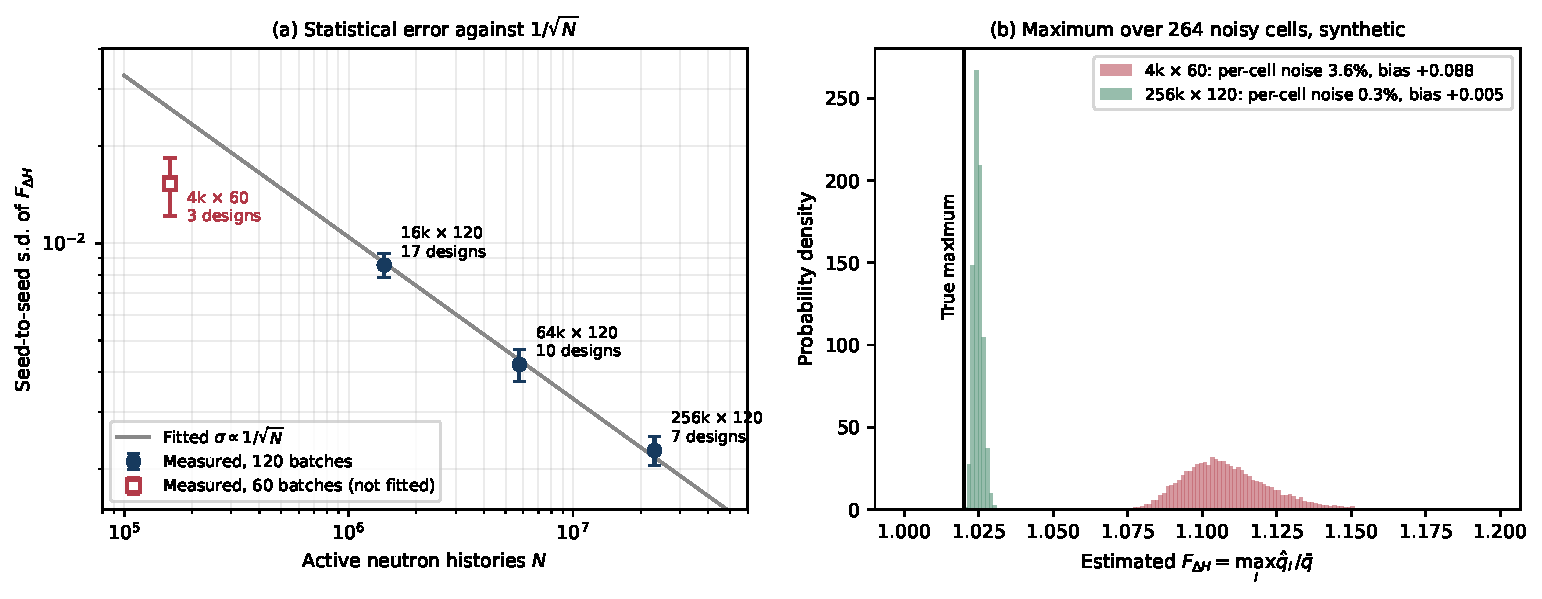
\includegraphics[width=\linewidth]{images/bg_mc_noise.pdf}
  \caption{Monte Carlo statistics of the peaking estimator.}
  \label{fig:bg-mc}
\end{figure}

\section{Reduced-order proxies and rank fidelity}
\label{sec:bg-proxy}

An optimiser driven by a cheap proxy inherits the \emph{ordering} that
the proxy imposes on candidate designs. Non-dominated sorting compares
designs pairwise, so any error that preserves the order of the designs,
such as a constant offset or scale factor, leaves the selection
unchanged. What matters for the search is therefore how well the proxy
ranks the designs, which a rank correlation measures. The absolute error
still matters wherever the proxy is compared with a fixed limit, as in a
constraint, and wherever its value is reported.

Spearman's rank correlation coefficient is used for that
purpose~\cite{kendall_gibbons_1990}. It is the Pearson correlation of
the two rankings, which for $n$ designs without tied values reduces to
Equation~\eqref{eq:spearman}.

\begin{equation}
\rho_S = 1 - \frac{6 \sum_{i=1}^{n} d_i^{\,2}}{n\,(n^{2}-1)}
\label{eq:spearman}
\end{equation}

\noindent where the symbols have the following meaning:

\begin{itemize}
  \item $\rho_S$ is Spearman's rank correlation coefficient,
        dimensionless, bounded between $-1$ and $+1$, equal to $+1$ for
        identical orderings. The subscript distinguishes it from
        reactivity, Equation~\eqref{eq:reactivity}.

  \item $d_i$ is the difference between the rank assigned to design $i$
        by the proxy and the rank assigned to the same design by the
        reference quantity, dimensionless.

  \item $n$ is the number of paired designs, dimensionless.

  \item $i$ is the design index, dimensionless.
\end{itemize}

The weakness of a rank-based proxy is systematic. Proxy-to-truth
correlation degrades near the optimum, where candidate designs crowd
together in objective space and small structural errors are enough to
reorder them.

Two responses to this problem exist in the literature, and both are
exercised in this thesis (Sections~\ref{sec:meth-core-objective}
and~\ref{sec:res-corevalidation}):

\begin{enumerate}
  \item Fuse the fidelities statistically, through a learned
        discrepancy between the cheap and the expensive
        model~\cite{kennedy_ohagan_2000,forrester_book_2008}.

  \item Measure the expensive quantity directly, wherever its cost
        permits.
\end{enumerate}

\section{The dual optimisation process}
\label{sec:bg-moo}

The optimisation of this thesis is built around a trade-off between two
costs: the cost of evaluating a design and the cost of searching for
good designs. One evaluation of the truth is a coupled OpenMC transport and depletion
calculation. It takes fifteen to twenty-five minutes, depending on the
campaign fidelity (Section~\ref{sec:meth-fidelity}).

A population-based search carries many candidate designs at once and
improves them collectively, without following a single trajectory. The
search used here, NSGA-II, is of that kind.

In Campaigns 1 to 5 NSGA-II evolved a population of 60 designs over 80
generations, which is 4800 objective evaluations for one search. From
Campaign 6 the population is 300 designs over 400 generations, or
\num{120000} evaluations. One such search is performed at every
iteration of the loop.

The change followed a sensitivity study before Campaign 6
(Section~\ref{sec:meth-nsga-setting}, Table~\ref{tab:nsga-sens}). The
surrogates were frozen on the Campaign 6 design of experiments, and
the search alone was repeated at six settings with eight seeds each:

\begin{itemize}
  \item At $60\times80$ the hypervolume of the surrogate front varied
        from seed to seed by a standard deviation of 12.7, about thirty
        per cent of the whole range covered by the six settings, so the
        selected designs depended on the seed.

  \item At $300\times400$ the hypervolume was the highest of the six and
        the seed-to-seed standard deviation fell to 0.6.

  \item The larger search costs about \SI{8}{\second}, which is
        negligible against one transport evaluation.
\end{itemize}

If each of the 4800 evaluations of the smaller search were an OpenMC
calculation, one search
alone would require seven to twelve weeks of continuous computation, and
a campaign of eight iterations between one and two years. Coupling the
search directly to the transport code is therefore computationally
prohibitive.

The resolution is a \emph{dual} process with two stages of very
different cost~\cite{forrester_book_2008}:

\begin{enumerate}
  \item An expensive \emph{evaluation} stage, in which OpenMC produces
        a small number of trusted data points.

  \item A cheap \emph{search} stage, in which a statistical model
        trained on those points is optimised in place of the code.
\end{enumerate}

Four components implement this process. The following subsections build
them in order of dependence:

\begin{enumerate}
  \item The hypervolume indicator, which measures the progress of a set
        of designs.

  \item The NSGA-II search, which produces such sets.

  \item The Gaussian-process surrogate, which makes the search
        affordable.

  \item The active-learning loop, which closes the cycle between search
        and evaluation.
\end{enumerate}

The four components share the concept of Pareto dominance, which is
defined first. With two competing objectives no single optimum exists, and the outcome of the
optimisation is a set of mutually incomparable designs.

Design $a$ \emph{dominates} design $b$ if it is at least as good as $b$
in both objectives and strictly better in at least one of
them~\cite{miettinen_1999,deb_2001}. The non-dominated subset of a design archive is its Pareto set, and the
corresponding attainment staircase in objective space is the Pareto
front, illustrated in Figure~\ref{fig:bg-pareto}.

Because the cycle length is maximised and $F_{\Delta H}$ is minimised,
the front appears there as a lower-right attainment staircase. The
reference point lies at the worst value of both objectives. Campaign~9
replaces the cycle length by the critical boron concentration
$c_\mathrm{max}$, and the cycle length becomes a constraint
(Section~\ref{sec:meth-c9}). Both objectives are then minimised, so
its front is a lower-left staircase and the reference point moves to
the upper right.

\begin{figure}[!tbp]
  \centering
  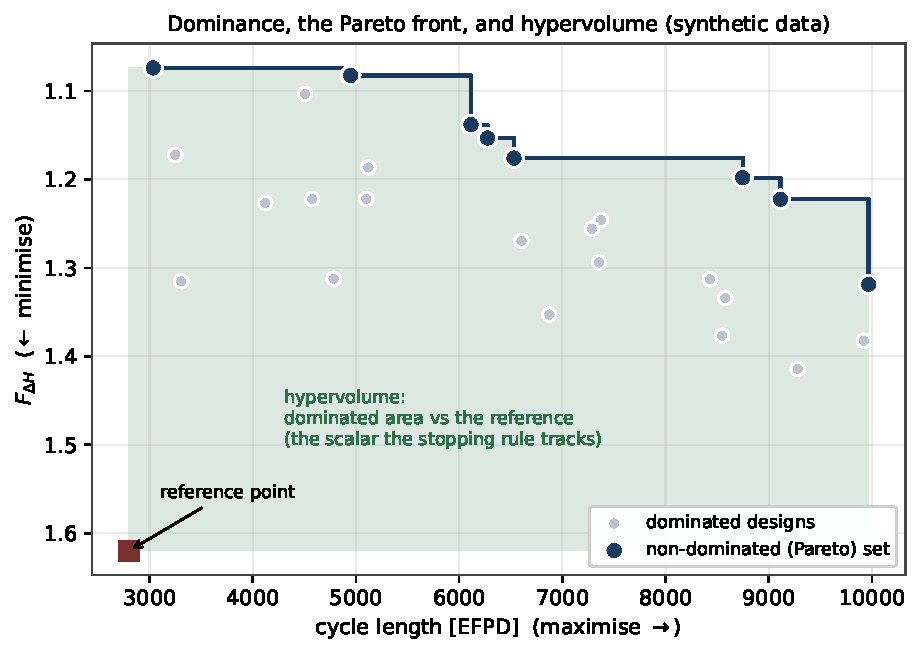
\includegraphics[width=0.82\linewidth]{images/bg_pareto_hv.pdf}
   \caption{Dominance, the Pareto front and the hypervolume.}
  \label{fig:bg-pareto}
\end{figure}

One sign convention simplifies everything that follows. Optimisation
libraries minimise by default, so the maximised objective of this
thesis, the cycle length, is negated internally and both objectives are
treated as minimisations.

All formulas below are written in that convention, and every reported
number is converted back before display.

\subsection{The hypervolume indicator}
\label{sec:bg-hv}

The search operates on \emph{sets} of designs, so its progress cannot
be tracked by watching a single number improve. The hypervolume
indicator solves this by compressing an entire Pareto front into one
scalar~\cite{coello_2007}.

\begin{equation}
\mathrm{HV}(\mathcal{P})
= \lambda\!\left( \bigcup_{\mathbf{f} \in \mathcal{P}}
  \left[\, \mathbf{f},\, \mathbf{r} \,\right] \right)
\label{eq:hv}
\end{equation}

\noindent where the symbols have the following meaning:

\begin{itemize}
  \item $\mathrm{HV}(\mathcal{P})$ is the hypervolume of the front
        $\mathcal{P}$, in the product of the objective units, for
        example EFPD times the dimensionless peaking factor in
        Campaigns 1 to 8 and the critical boron concentration, in ppm,
        times the peaking factor in Campaign~9.

  \item $\lambda$ is the Lebesgue measure, which for two objectives is
        simply the area.

  \item $\mathcal{P}$ is the set of objective vectors of the
        non-dominated designs.

  \item $\mathbf{f}$ is the objective vector of one front member, with
        one coordinate per objective.

  \item $\mathbf{r}$ is the reference point, a fixed objective vector
        chosen worse than every front member in every objective.

  \item $[\mathbf{f}, \mathbf{r}]$ is the axis-aligned rectangle
        spanned by $\mathbf{f}$ and $\mathbf{r}$, that is, the region
        of objective space dominated by that member relative to the
        reference.
\end{itemize}

Figure~\ref{fig:bg-hv-construction} illustrates the construction on a
schematic front, not on campaign data. Its four panels correspond to
the four steps below:

\begin{enumerate}
  \item Fix the reference point once, at a value worse than any design
        of interest in both objectives.

  \item For each front member, draw the rectangle between the member
        and the reference point. Everything inside that rectangle is
        dominated by the member.

  \item Take the union of the rectangles. Overlaps are counted once.

  \item The area of the union is the hypervolume.
\end{enumerate}

\begin{figure}[!tbp]
  \centering
  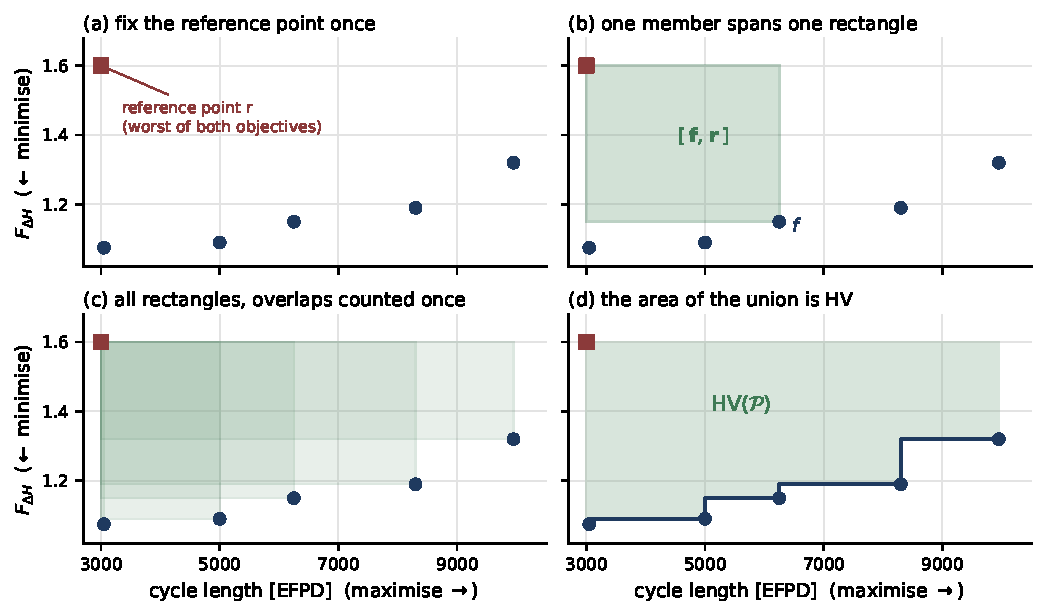
\includegraphics[width=\linewidth]{images/bg_hv_construction.pdf}
  \caption{Illustrative construction of the hypervolume.}
  \label{fig:bg-hv-construction}
\end{figure}

Two properties make the indicator the right convergence diagnostic:

\begin{enumerate}
  \item It respects Pareto dominance. When one front is better than
        another, its hypervolume is strictly larger, because the better
        front dominates a region of objective space that the other does
        not~\cite{zitzler_2003_performance}.

  \item It rewards both convergence and spread, because a front that
        covers a wider range of trade-offs dominates a larger region.
\end{enumerate}

Figure~\ref{fig:bg-hv-gain} shows the only two mechanisms by which the
indicator can grow. Of the two designs added at iteration $k+1$, one
pushes the front outward and the other fills a gap.

\begin{figure}[htbp]
  \centering
  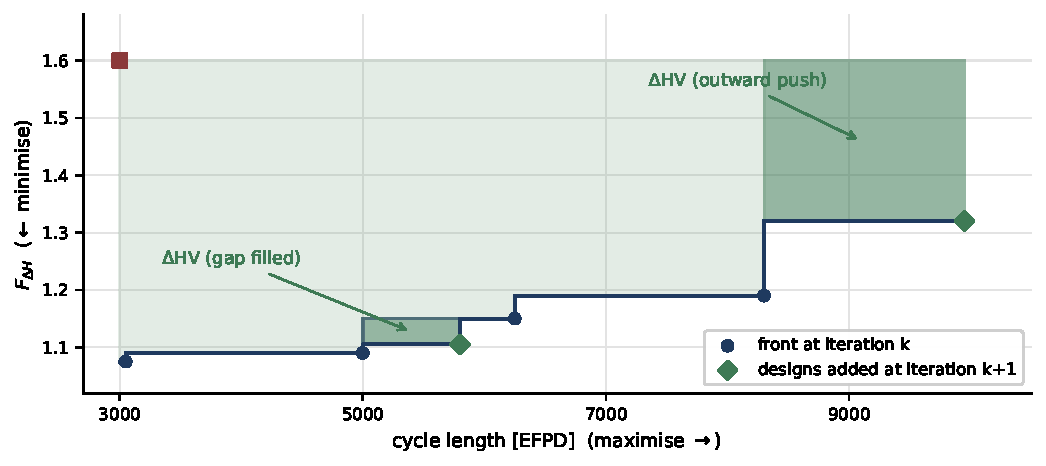
\includegraphics[width=0.9\linewidth]{images/bg_hv_gain.pdf}
  \caption{Growth of the hypervolume between two iterations.}
  \label{fig:bg-hv-gain}
\end{figure}

The indicator carries one obligation in exchange for its convenience.
Its numerical value depends on the reference point and on the units of
the objectives as much as on the front itself.

The dependence is shown below on one unchanged front measured from three
reference points. The front is the illustrative five-member front of
Figure~\ref{fig:bg-hv-construction}, not the front of any campaign, so
the values below do not appear in Chapter~\ref{ch:results}. The first
reference point is the one drawn in that figure. The other two are
alternatives that could
equally have been chosen, and are not shown:

\begin{itemize}
  \item $\mathbf{r} = (3000~\mathrm{EFPD},\, 1.60)$, the value used in
        Figure~\ref{fig:bg-hv-construction}, gives
        $\mathrm{HV} = 2886$.

  \item $\mathbf{r} = (2500~\mathrm{EFPD},\, 1.80)$, a more permissive
        corner, gives $\mathrm{HV} = 4638$.

  \item $\mathbf{r} = (3000~\mathrm{EFPD},\, 1.45)$, a stricter corner,
        gives $\mathrm{HV} = 1843$.
\end{itemize}

No design has moved between the three cases. The front is identical in
all of them, and the reported value still varies by a factor of two and
a half.

The choice of units has the same effect. The hypervolume of a
two-objective problem has the units of the product of its objectives,
for example effective full-power days multiplied by a dimensionless
factor. Reporting cycle length in years instead of days divides every
value by 365.25 without changing a single design, so an isolated
hypervolume states nothing about the quality of a front.

What carries meaning is the change in hypervolume between two
iterations, measured against the same reference point. The change is
the area of the region that the new front dominates and the previous
front did not. It is therefore positive only when a new design has moved
the front outward or filled a gap between its members, and zero when
the front is unchanged.

The stopping rule of Section~\ref{sec:meth-loop} therefore uses the gain
relative to the previous hypervolume, below \SI{1}{\percent} for three
consecutive iterations, and not an absolute value of the hypervolume. A
change of units multiplies the gain and the previous hypervolume by the
same factor, so their ratio is unchanged, while an absolute threshold
would have to be chosen again for every choice of units. The ratio still
depends on the reference point, because the reference point sets the
area credited to the extreme members of the front. The reference point
is therefore kept fixed within a campaign, as the rules below require.

Two rules of comparability follow, and both are respected throughout
this work:

\begin{enumerate}
  \item Within one campaign the reference point is fixed once and never
        revised, so every value in the history is comparable to every
        other.

  \item Across campaigns the values are not comparable whenever the
        reference point or the definition of an objective has changed,
        and no such comparison is drawn in Chapter~\ref{ch:results}.
\end{enumerate}

\subsection{The NSGA-II search}
\label{sec:bg-nsga2}

The Non-dominated Sorting Genetic Algorithm II
(NSGA-II)~\cite{deb_nsga2_2002} is the engine that produces candidate
Pareto sets. It belongs to the family of genetic algorithms, which
mimic natural selection on a population of candidate
solutions~\cite{deb_2001}.

Each design is an individual, its design vector plays the role of its
genes, and better individuals are given more descendants.

A genetic algorithm iterates four operations:

\begin{enumerate}
  \item \emph{Selection.} Better candidates are given a higher chance
        of becoming parents.

  \item \emph{Crossover.} Pairs of parents are recombined into
        offspring, the new candidate designs, whose variables combine the
        values of both parents. This work uses simulated binary
        crossover, the default operator of the NSGA-II implementation
        adopted~\cite{deb_2001,blank_deb_2020}.

  \item \emph{Mutation.} Small random perturbations keep the population
        from collapsing prematurely.

  \item \emph{Replacement.} The next generation is formed and the cycle
        repeats.
\end{enumerate}

The step that does not survive the move to two objectives is the first
one, because ``better'' is no longer a single number. A design with a
longer cycle and a design with a lower peaking factor are each better
than the other in one respect, and the same holds in Campaign~9 for a
design with a lower critical boron concentration and a design with a
lower peaking factor.

NSGA-II resolves this with two rankings computed on the current
population~\cite{deb_nsga2_2002,deb_2001}:

\begin{itemize}
  \item Non-dominated sorting, which measures quality.

  \item The crowding distance, which measures diversity.
\end{itemize}

\subsubsection*{Comparing two designs}

The basic comparison is the dominance of Section~\ref{sec:bg-moo}, and
Figure~\ref{fig:bg-nsga2-sorting}(a) shows everything it can say. Any
design $X$ splits the objective plane into four quadrants:

\begin{enumerate}
  \item Designs that are at least as good in both objectives and
        strictly better in at least one \emph{dominate} $X$, as $A$ does
        in Figure~\ref{fig:bg-nsga2-sorting}(a).

  \item Designs that are at least as bad in both, one strictly, are
        \emph{dominated by} $X$, as $B$ is.

  \item Designs in the two remaining quadrants trade one objective
        against the other. They are \emph{incomparable} with $X$, and
        dominance is silent about them.
\end{enumerate}

Incomparability states that, between a longer cycle and a flatter power
distribution, no preference has been imposed yet. Near a Pareto front
almost every pair of designs is incomparable, which is exactly why a
second ranking is needed.

\subsubsection*{Non-dominated sorting}

The first ranking turns dominance into an integer grade for every
design, by removing successive non-dominated fronts.

\begin{enumerate}
  \item Find every design that no other design dominates. These form
        \emph{rank 1}, the current best front.

  \item Set rank 1 aside and repeat the test on the remainder. The
        designs now dominated by nobody form \emph{rank 2}.

  \item Continue until every design has been assigned to a rank.
\end{enumerate}

The rank of a design therefore counts how many fronts must be removed
before that design becomes non-dominated, and
Figure~\ref{fig:bg-nsga2-sorting}(b) shows a population sorted into
four ranks. The ranks obey three rules:

\begin{itemize}
  \item Every design receives exactly one rank.

  \item A lower rank is always preferred.

  \item Designs of the same rank are mutually incomparable.
\end{itemize}

\begin{figure}[!tbp]
  \centering
  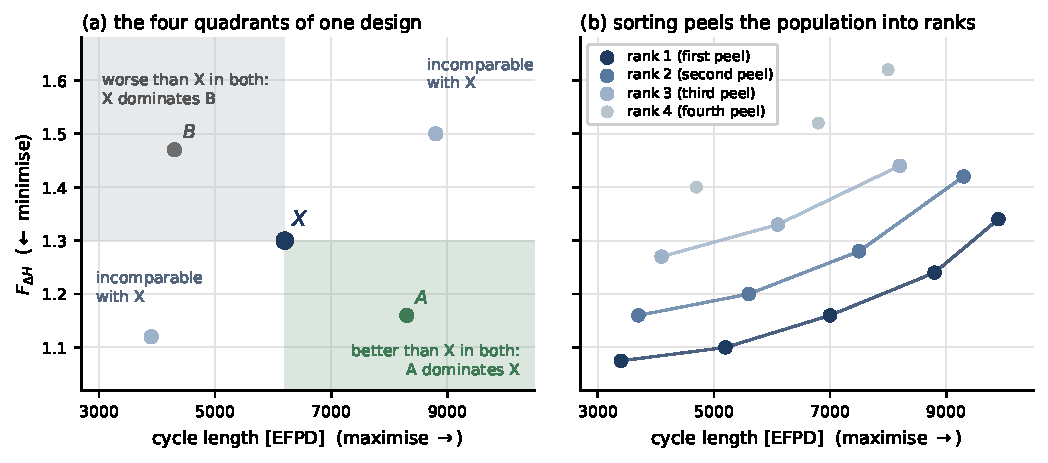
\includegraphics[width=\linewidth]{images/bg_nsga2_sorting.pdf}
  \caption{Dominance and non-dominated sorting.}
  \label{fig:bg-nsga2-sorting}
\end{figure}

\subsubsection*{Crowding distance}

The second ranking is a secondary selection criterion among designs of
the same rank, and it preserves the diversity of the population. It uses
the \emph{crowding distance}, a density estimate that measures how
isolated a design is from its neighbours along the front, and designs
are compared through the crowded-comparison
operator~\cite{deb_nsga2_2002}.

\begin{equation}
d_i = \sum_{m=1}^{M}
\frac{f_m^{(i+1)} - f_m^{(i-1)}}{f_m^{\max} - f_m^{\min}}
\label{eq:crowding}
\end{equation}

\noindent where the symbols have the following meaning:

\begin{itemize}
  \item $d_i$ is the crowding distance of design $i$, dimensionless,
        because each summand is normalised.

  \item $M$ is the number of objectives, equal to 2 in this thesis.

  \item $f_m^{(i+1)}$ and $f_m^{(i-1)}$ are the values of objective $m$
        for the two neighbours of design $i$ when its rank is sorted
        along that objective, in the units of objective $m$.

  \item $f_m^{\max}$ and $f_m^{\min}$ are the extreme values of
        objective $m$ within the rank, in the same units.

  \item The two boundary designs of each rank receive an infinite
        crowding distance, so the extremes of the front are never
        discarded.
\end{itemize}

Geometrically, $d_i$ is the normalised perimeter of the box spanned by
the two neighbours of design $i$, shown in
Figure~\ref{fig:bg-nsga2-crowding}.

A design in a sparsely populated stretch of the front has distant
neighbours, a large box and a large $d_i$. Keeping it preserves a
trade-off option that no other design represents. A design inside a
tight cluster is nearly redundant and is the first to be discarded.

Selection then follows one rule with one tie-breaker:

\begin{enumerate}
  \item The lower rank wins.

  \item At equal rank, the larger crowding distance wins.
\end{enumerate}

\begin{figure}[!tbp]
  \centering
  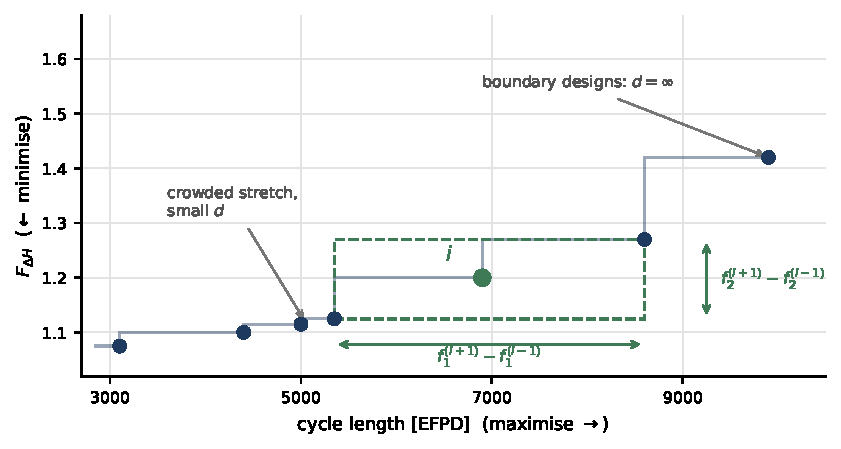
\includegraphics[width=0.8\linewidth]{images/bg_nsga2_crowding.pdf}
  \caption{Crowding distance of Equation~\eqref{eq:crowding}.}
  \label{fig:bg-nsga2-crowding}
\end{figure}

\subsubsection*{Constrained domination}

A constrained problem adds a difficulty. Most designs the search
generates violate at least one constraint, and simply discarding them
would leave selection with nothing to act on.

In the extreme case of a population with no feasible member at all,
discarding infeasible designs leaves no design to rank. The selection
operator then has no basis for preferring one design over another, and
the search loses all selection pressure. NSGA-II instead extends
dominance so that any two designs can always be compared, using the
total constraint violation~\cite{deb_nsga2_2002}.

\begin{equation}
V(\mathbf{x}) = \sum_{j=1}^{n_g} \max\bigl( 0,\, g_j(\mathbf{x}) \bigr)
\label{eq:violation}
\end{equation}

\noindent where the symbols have the following meaning:

\begin{itemize}
  \item $V(\mathbf{x})$ is the total constraint violation of design
        $\mathbf{x}$, dimensionless, equal to zero exactly when the
        design is feasible.

  \item $g_j(\mathbf{x})$ is the $j$-th constraint of
        Table~\ref{tab:constraints} in normalised form, dimensionless,
        feasible when non-positive.

  \item $n_g$ is the number of active inequality constraints of the
        campaign, dimensionless. It changes between campaigns, as stated
        with Equation~\eqref{eq:constraint_form}.

  \item $\max(0, \cdot)$ keeps only the violated part, so satisfied
        constraints contribute nothing and cannot compensate for
        violated ones.
\end{itemize}

\emph{Constrained domination} compares any pair of designs by three
rules, applied in order, restating Definition~1 of
Deb et al.~\cite{deb_nsga2_2002}:

\begin{enumerate}
  \item A feasible design always beats an infeasible one.

  \item Between two infeasible designs, the smaller total violation
        $V$ wins. Objective values are ignored.

  \item Between two feasible designs, Pareto dominance decides,
        %
        \begin{equation}
        \begin{split}
          \mathbf{x}^{(a)} \prec \mathbf{x}^{(b)}
          \iff
          & \forall i \in \{1,2\} :
            f_i\bigl(\mathbf{x}^{(a)}\bigr) \le f_i\bigl(\mathbf{x}^{(b)}\bigr) \\
          & \wedge\
            \exists j \in \{1,2\} :
            f_j\bigl(\mathbf{x}^{(a)}\bigr) < f_j\bigl(\mathbf{x}^{(b)}\bigr)
        \end{split}
        \label{eq:pareto-dominance-feasible}
        \end{equation}
        %
        The symbols carry the following meaning.
        \begin{itemize}
          \item $\mathbf{x}^{(a)}, \mathbf{x}^{(b)}$: two feasible
                design vectors, dimensionless.
          \item $\prec$: the dominance relation, read as
                \emph{dominates}, dimensionless.
          \item $f_1$: the cycle length in Effective Full Power Days
                (EFPD), negated so that maximisation becomes
                minimisation, in days.
          \item $f_2$: the radial enthalpy-rise hot-channel factor
                $F_{\Delta H}$, dimensionless.
          \item $i, j$: objective indices, dimensionless.
        \end{itemize}
        If neither design dominates the other, the two are mutually
        non-dominated. The crowded-comparison operator then prefers the
        design of lower non-domination rank and, at equal rank, the
        design with the larger crowding distance of
        Equation~\eqref{eq:crowding}~\cite{deb_nsga2_2002}.
\end{enumerate}

Figure~\ref{fig:bg-nsga2-thesis}(a) shows the three rules acting on a
mixed population. Rule 2 keeps a fully infeasible population
completely ordered, so selection still moves toward the feasible
region instead of stalling.

\begin{figure}[!tbp]
  \centering
  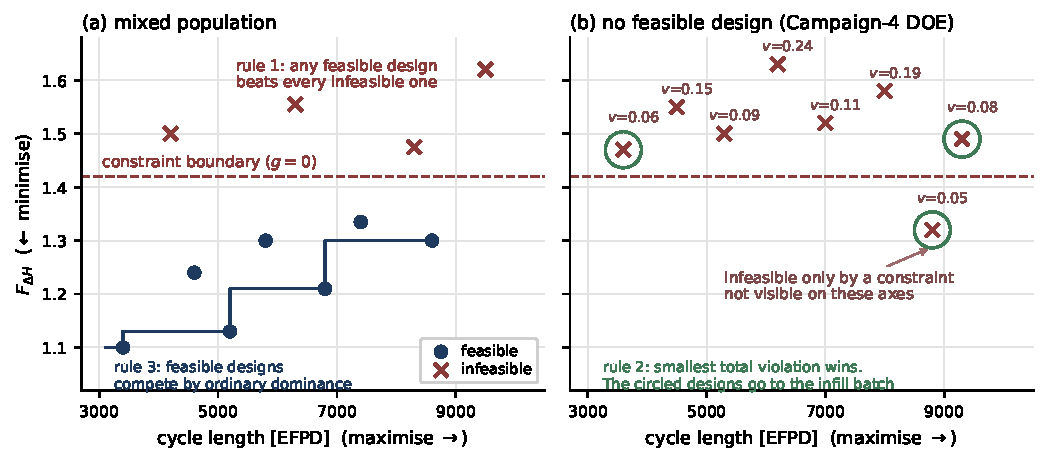
\includegraphics[width=\linewidth]{images/bg_nsga2_thesis.pdf}
  \caption{Constrained domination on illustrative data.}
  \label{fig:bg-nsga2-thesis}
\end{figure}

\subsubsection*{One generation}
With the comparisons in place, one elitist generation of NSGA-II
follows the main loop of Deb et al.~\cite{deb_nsga2_2002}.
Figure~\ref{fig:bg-nsga2-generation}, adapted from Figure~2 of that
paper, traces it:

\begin{enumerate}
  \item Create the offspring population $Q_t$ from the parent
        population $P_t$ of size $N$ by binary tournament selection
        under the comparisons above, followed by crossover and
        mutation.
  \item Pool parents and offspring into $R_t = P_t \cup Q_t$, $2N$
        designs in total. Every parent competes again, so the best
        designs found so far cannot be lost. This is the elitism of
        the algorithm.
  \item Sort $R_t$ into fronts $F_1, F_2, \ldots$ by non-dominated
        sorting under constrained domination.
  \item Fill the next population $P_{t+1}$ front by front until a
        front no longer fits entirely.
  \item Fill the remaining places from that first overfull front, $F_3$
        in the figure, in decreasing order of crowding distance. Reject
        the rest of that front and all lower fronts.
  \item Repeat until the generation budget is exhausted. The first
        front of the final population is the candidate Pareto set.
\end{enumerate}

\begin{figure}[!tbp]
  \centering
  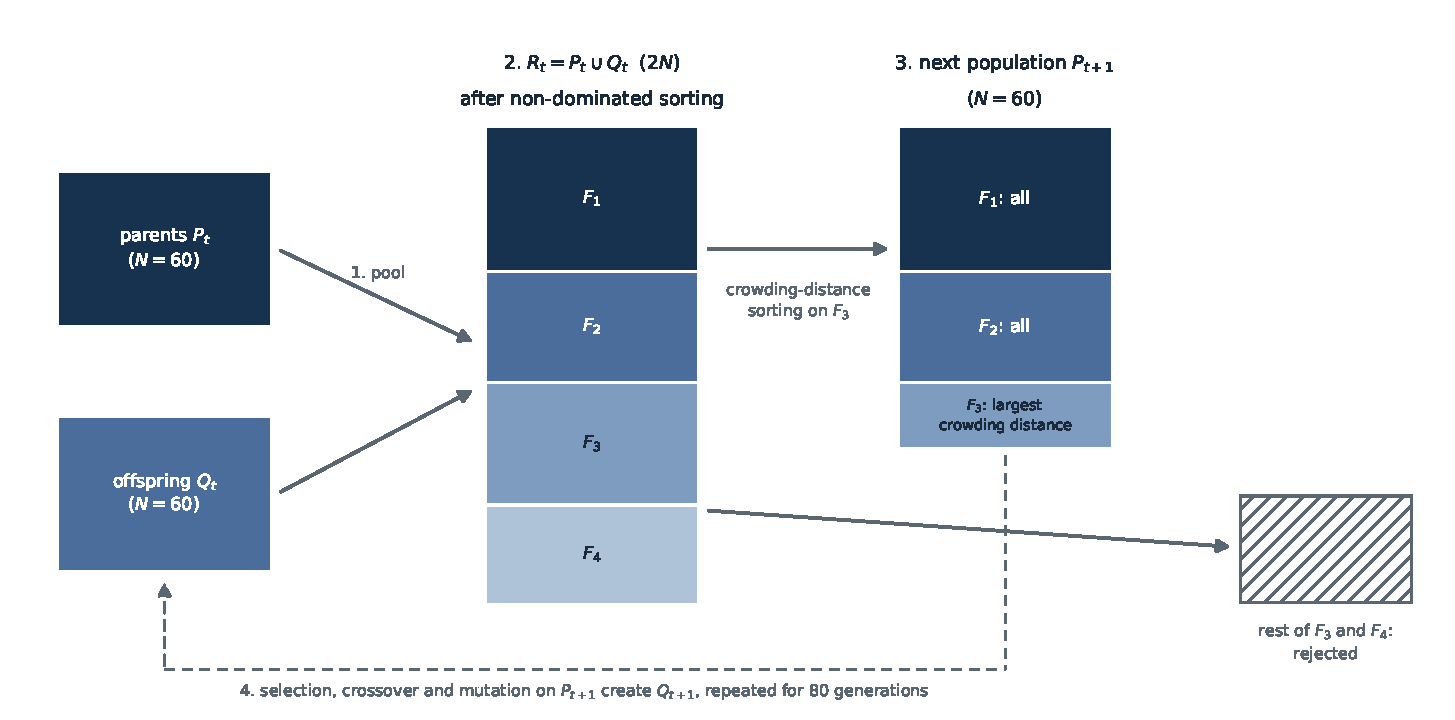
\includegraphics[width=0.95\linewidth]{images/bg_nsga2_generation.pdf}
  \caption[One elitist generation of NSGA-II]{One elitist generation of NSGA-II.\newline Figure adapted from~\cite{deb_nsga2_2002}.}
  \label{fig:bg-nsga2-generation}
\end{figure}

The population is defined by the settings of the campaign:

\begin{itemize}
  \item It lives in the design space of Table~\ref{tab:design-space},
        handled internally on the unit hypercube.

  \item It is judged on the two objectives of
        Section~\ref{sec:objective_functions}, with EFPD negated.

  \item It is subject to the constraints of Table~\ref{tab:constraints}
        in the $g \le 0$ convention that
        Equation~\eqref{eq:violation} consumes.
\end{itemize}

The number of design variables and the number of constraints both
change between campaigns. The values of each campaign are those of
Equation~\eqref{eq:constraint_form}.

NSGA-II never calls OpenMC. Each active-learning iteration searches
the Gaussian-process surrogate of Section~\ref{sec:bg-gp} with a
population of 300 evolved for 400 generations from Campaign 6, and of
60 for 80 generations before it (Section~\ref{sec:meth-nsga-setting}),
initialised by Latin hypercube sampling with a fresh random seed. One complete search
therefore costs seconds, instead of the thousands of transport
evaluations it replaces.

Constrained domination also kept the search alive at the Campaign-4
design of experiments, where all 36 designs were infeasible and
selection was governed entirely by rule 2. The final population is then
ranked by total violation, and its least-infeasible members are handed
to the infill step. This is the constraint-violation-driven mode of
Section~\ref{sec:res-c4}, drawn in Figure~\ref{fig:bg-nsga2-thesis}(b).

In that figure, the design with $V = 0.05$ lies below the dashed
boundary on $F_{\Delta H}$ and would look feasible if only its position
in the objective plane were inspected. It is infeasible nonetheless,
because it violates a constraint on a quantity that is not an
objective. Most constraints of Table~\ref{tab:constraints} act on such
quantities, among them the beginning-of-life multiplication factor and
the enrichment cap. The feasibility of a design, and its total violation
$V$, therefore cannot be inferred from its position in the objective
plane, and $V$ is computed from every constraint of the table.

\FloatBarrier


\subsection{Gaussian-process surrogates}
\label{sec:bg-gp}

A surrogate is a statistical stand-in for the expensive code, trained
on the designs evaluated so far and consulted everywhere
else~\cite{forrester_book_2008}. The search of the previous subsection
needs thousands of evaluations per iteration, and the surrogate is what
makes them affordable.

A Gaussian process (GP) is the surrogate family used here. Before any
design is evaluated, the GP treats the unknown objective as a random
function, and this prior distribution over functions expresses what is
assumed about the objective in advance. The prior is specified
completely by two functions~\cite{rasmussen_gp_2006}:

\begin{itemize}
  \item The mean function, the value expected at any design before data
        are available.

  \item The covariance kernel, which states how strongly the outputs of
        two designs are expected to vary together, as a function of
        their distance in the design space.
\end{itemize}

Conditioning the GP on the evaluated designs updates the prior with
Bayes' rule, so that the distribution becomes consistent with the
observed results. The updated distribution is the posterior. Its mean is
the prediction of the surrogate, and with the noise term used in this
work it passes close to, not exactly through, the evaluated values. Its
variance is the uncertainty of that prediction. It is small near
evaluated designs and grows with the distance from them, where the data
constrain the function least~\cite{rasmussen_gp_2006}.

Figure~\ref{fig:bg-gp} illustrates the posterior mean and variance,
together with the growth of the predictive uncertainty away from the
data that active learning exploits. The reasoning proceeds in four steps:

\begin{enumerate}
  \item Assume similarity: designs that are close in the design space
        should produce similar objective values.

  \item Encode that assumption in a kernel $k(\mathbf{x},\mathbf{x}')$,
        a function that returns the assumed covariance between the
        outputs of two designs from their distance.

  \item Condition on the archive of evaluated designs, that is, update
        the prior with the OpenMC results of every design evaluated so
        far, so that the predictions become consistent with them.

  \item Evaluate the posterior predictive distribution at any untried
        design, which gives its predicted mean and its predictive
        standard deviation.
\end{enumerate}

The kernel used in this work is the anisotropic Mat\'ern covariance
with smoothness $\nu = 5/2$, plus a white-noise
term~\cite{rasmussen_gp_2006}. Each of its three features answers a
property of the problem:

\begin{itemize}
  \item The Mat\'ern form with $\nu = 5/2$ gives functions that are twice
        differentiable. The squared-exponential kernel, the other common
        choice, gives infinitely differentiable functions, a smoothness
        that is considered unrealistic for most physical
        responses~\cite{rasmussen_gp_2006}.

  \item The anisotropy assigns one length scale to each design variable,
        because enrichment, gadolinia content, poisoned-pin count and
        reflector thickness change the objectives at different rates.

  \item The white-noise term represents the Monte Carlo noise of every
        evaluation, so the posterior mean is not forced through noisy
        values.
\end{itemize}

The choice follows common practice and was not compared against other
kernels in this work.

\begin{equation}
k(\mathbf{x}, \mathbf{x}')
= \sigma_f^{2}
\left( 1 + \sqrt{5}\,r + \tfrac{5}{3}\,r^{2} \right)
\exp\!\left( -\sqrt{5}\,r \right)
+ \sigma_n^{2}\,\delta_{\mathbf{x}\mathbf{x}'}
\label{eq:kernel}
\end{equation}

\begin{equation}
r = \left[ \sum_{d=1}^{D}
\frac{(x_d - x'_d)^{2}}{\ell_d^{\,2}} \right]^{1/2}
\label{eq:kernel-r}
\end{equation}

\noindent where the symbols have the following meaning:

\begin{itemize}
  \item $k(\mathbf{x}, \mathbf{x}')$ is the covariance between the
        outputs at designs $\mathbf{x}$ and $\mathbf{x}'$, in the
        squared units of the modelled output.

  \item $\sigma_f^{2}$ is the signal variance, in the squared units of
        the output, setting the overall scale of variation.

  \item $r$ is the scaled distance between the two designs,
        dimensionless.

  \item $x_d$ and $x'_d$ are the $d$-th components of the two design
        vectors after standardisation, dimensionless.

  \item $D$ is the number of design variables, equal to 5 in Campaigns
        1 to 4.

  \item $\ell_d$ is the length-scale of variable $d$, dimensionless
        after standardisation. One length-scale per variable is the
        automatic relevance determination (ARD) structure.

  \item $\sigma_n^{2}$ is the noise variance, in the squared units of
        the output, absorbing the evaluation noise.

  \item $\delta_{\mathbf{x}\mathbf{x}'}$ is the Kronecker delta, equal
        to 1 when the two designs coincide and 0 otherwise,
        dimensionless.
\end{itemize}

Conditioning the prior on $n$ archive evaluations gives the posterior
prediction at any new design $\mathbf{x}$~\cite{rasmussen_gp_2006}.

\begin{equation}
\mu_*(\mathbf{x})
= \mathbf{k}_*^{\mathsf T}
\left( \mathbf{K} + \sigma_n^{2}\,\mathbf{I} \right)^{-1} \mathbf{y}
\label{eq:gp-mean}
\end{equation}

\begin{equation}
\sigma_*^{2}(\mathbf{x})
= k(\mathbf{x}, \mathbf{x})
- \mathbf{k}_*^{\mathsf T}
\left( \mathbf{K} + \sigma_n^{2}\,\mathbf{I} \right)^{-1} \mathbf{k}_*
\label{eq:gp-var}
\end{equation}

\noindent where the symbols have the following meaning:

\begin{itemize}
  \item $\mu_*(\mathbf{x})$ is the predicted mean at design
        $\mathbf{x}$, in the units of the output.

  \item $\sigma_*^{2}(\mathbf{x})$ is the predictive variance of the
        underlying response at $\mathbf{x}$, in the squared units of
        the output.

  \item $\mathbf{y}$ is the vector of the $n$ archive outputs, in the
        units of the output.

  \item $\mathbf{K}$ is the $n \times n$ matrix of kernel values
        between archive designs, with entries
        $K_{ij} = k(\mathbf{x}_i, \mathbf{x}_j)$.

  \item $\mathbf{k}_*$ is the vector of kernel values between the new
        design and each archive design, with entries
        $k(\mathbf{x}_i, \mathbf{x})$.

  \item $\mathbf{I}$ is the $n \times n$ identity matrix,
        dimensionless.

  \item $n$ is the number of archive evaluations, dimensionless.
\end{itemize}

The two equations have a simple reading~\cite{rasmussen_gp_2006}:

\begin{itemize}
  \item Equation~\eqref{eq:gp-mean} says the prediction is a weighted
        average of the archive outputs, with weights set by similarity.

  \item Equation~\eqref{eq:gp-var} says the uncertainty shrinks near
        evaluated designs and grows away from them, which is exactly the
        information the active-learning loop consumes.
\end{itemize}

Two kernel features carry particular weight in this work:

\begin{enumerate}
  \item The ARD structure learns one length-scale per design variable.
        A variable along which the response is flat is assigned a large
        length-scale, so the fitted length-scales rank the variables by
        their influence on each output.

  \item The white-noise component absorbs the evaluation noise. Two
        properties of this component matter:
        \begin{enumerate}
          \item its assumption of independent and identically
                distributed noise across designs is violated by a
                shared random seed, which motivates the per-design
                seeding policy adopted in Campaign~3,
          \item its fitted magnitude is an upper bound on the true
                Monte Carlo noise, so the excess over the measured
                noise quantifies residual model misfit.
        \end{enumerate}
\end{enumerate}

\begin{figure}[htbp]
  \centering
  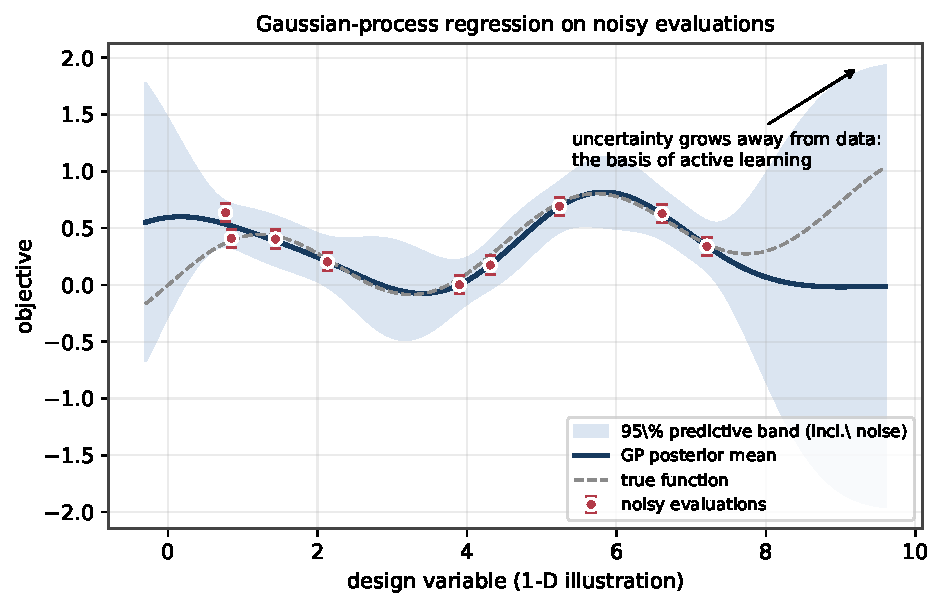
\includegraphics[width=0.8\linewidth]{images/bg_gp.pdf}
  \caption{Gaussian-process regression on noisy evaluations: posterior mean and 95\% predictive band.}
  \label{fig:bg-gp}
\end{figure}

The settings with which this surrogate is used in the campaigns are
fixed in Section~\ref{sec:meth-loop-settings}. They cover the
standardisation of inputs and outputs, one Gaussian process per output,
and the refitting of the hyperparameters at every iteration.

\subsection{The active-learning loop}
\label{sec:bg-al}

The surrogate is only as good as its training set, and the training set
is expensive. Active learning is the strategy of spending the
evaluation budget where it teaches the model
most~\cite{forrester_book_2008}.

The starting set must cover the design space before anything is known
about it. The initial design of experiments uses Latin hypercube
sampling (LHS)~\cite{mckay_lhs_1979}, built in three steps:

\begin{enumerate}
  \item The range of every variable is divided into as many equal
        slices as there are samples.

  \item Exactly one sample is placed in each slice of each variable.

  \item The combinations are randomly permuted.
\end{enumerate}

The guarantee is one-dimensional coverage: no variable is left with an
unexplored stretch. Uniform random sampling cannot promise that at
equal budget.

From there the campaign follows the dual-stage loop of
Figure~\ref{fig:bg-al}, whose steps repeat until the stopping rule is
met:

\begin{enumerate}
  \item Draw the LHS design of experiments and evaluate it with OpenMC,
        the expensive truth of Section~\ref{sec:meth-fidelity}.

  \item Fit the Gaussian-process surrogates of
        Section~\ref{sec:bg-gp}, objectives and constraints, on the
        whole cumulative archive and not on the newest batch alone.

  \item Run the NSGA-II search of Section~\ref{sec:bg-nsga2} on the
        surrogate. Its final rank-1 population is the candidate set.
        If the surrogate predicts no feasible region, the
        least-infeasible members take that role.

  \item Select the infill batch, the designs that are evaluated with
        OpenMC in this iteration, from the candidates. The selection
        proceeds in five sub-steps, detailed in
        Section~\ref{sec:meth-acq}:
        %
        \begin{enumerate}[label=\arabic{enumi}.\arabic*]
          \item Predict, for every candidate, the posterior standard
                deviation of each of the two objectives with
                Equation~\eqref{eq:gp-var}.

          \item Divide each standard deviation by the largest value of
                the same objective over the candidate set. The two
                objectives have different units, and the division gives
                them equal weight.

          \item Add the two normalised values. The sum is the
                uncertainty score of the candidate, and a high score
                marks a design whose predicted objectives rest on few
                nearby evaluations.

          \item Screen the candidates on the constraint surrogates.
                Candidates whose predicted constraints stay satisfied
                after a margin of $\kappa$ standard deviations rank first,
                by descending score. The others follow, from the least to
                the most likely to violate a constraint.

          \item Walk down the ranking and accept a candidate only if it
                lies at least a minimum normalised distance from every
                design of the archive and from the designs already
                accepted, which also excludes designs already evaluated.
                The walk stops when the batch is full. If the ranking runs
                out first, the minimum distance is halved and the walk is
                repeated.
        \end{enumerate}

        The candidate set and the uncertainty ranking play complementary
        roles:

        \begin{itemize}
          \item The candidate set supplies the \emph{exploitation}.
                Every candidate belongs to the rank-1 set of the surrogate
                search, so each is predicted to be among the best designs
                available.

          \item The uncertainty ranking supplies the
                \emph{exploration}. Among these promising designs, it
                sends to OpenMC those whose predictions are least
                supported by the data, so each evaluation tests a
                promising region and reduces the uncertainty where it is
                largest.
        \end{itemize}

  \item Evaluate the infill batch with OpenMC and append it to the
        archive.

  \item Record the state of the loop at the end of the iteration:
        %
        \begin{enumerate}[label=\arabic{enumi}.\arabic*]
          \item Recompute the hypervolume of Section~\ref{sec:bg-hv} on
                the updated archive.

          \item Write a checkpoint, a file holding the full archive of
                evaluated designs and their results.

          \item If the run is interrupted, for example by a machine
                failure, a loss of power or a software error, restart it
                from the last checkpoint.
        \end{enumerate}

        Only the OpenMC evaluations of the iteration in progress are
        lost, at most one infill batch, and no completed evaluation has
        to be repeated. The checkpoint was introduced after a crash
        during Campaign~4 discarded six completed evaluations.

  \item Between blocks of iterations, apply the stopping rule of
        Section~\ref{sec:meth-loop}. At convergence, pass the finalists
        to the high-fidelity confirmation of
        Section~\ref{sec:meth-stats}.
\end{enumerate}

The separation between a cheap search stage and an expensive
confirmation stage is the two-tier principle that recurs throughout the
thesis.

\begin{figure}[htbp]
  \centering
  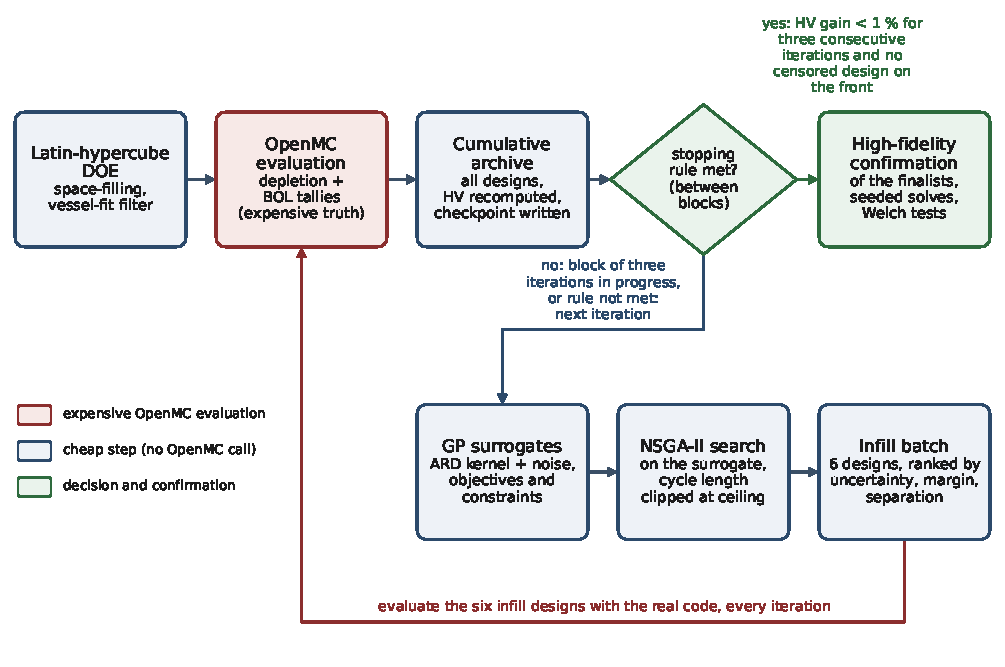
\includegraphics[width=0.95\linewidth]{images/bg_al_loop.pdf}
  \caption{The dual-stage surrogate-assisted active-learning loop as implemented.}
  \label{fig:bg-al}
\end{figure}

The design of experiments, the infill batch, the block structure and the
budget with which the loop was run are fixed in
Section~\ref{sec:meth-loop-settings}. They are stated once there, next
to the acquisition function they feed.
